\chapter{Test of DALI Zensor 5}
This section will go through a test of a loudspeaker to understand if any vibrations in the loudspeaker affect the distortion of the loudspeaker.
The loudspeaker which will be the basis for the test is the Zensor 5 (as seen on \autoref{fig:dali_zensor5}) given by DALI. A passive speaker has been choosen for the test because the amplifiers in DALI's active speakers are designed not to stress the loudspeaker to its limits and beyond, and to be able to test how the vibrations affect distortion, the loudspeaker must be tested to its limits and beyond.

\begin{figure}[H]
\centering
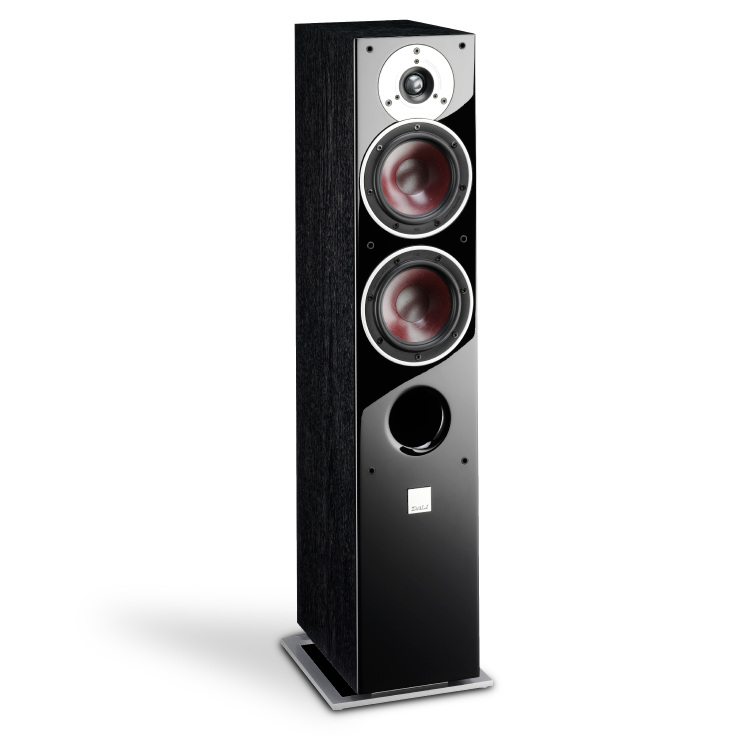
\includegraphics[width=0.5\textwidth]{figures/zensor5.png}
\caption{DALI zensor 5.}
\label{fig:dali_zensor5}
\end{figure}

\todo[inline]{Reference http://www.dali-speakers.com/loudspeakers/zensor/zensor-5/}

For measuring the vibrations inside the enclosure two accelometers have been placed inside the enclosure, one on the back of bottom driver and one on the top back of the enclosure. For measuring distortion a microphone has been placed 1 m from the speaker. To limit any reflection from a room for example, the test is perfomed in the Anechoic room at \gls{AAU} see \ref{fig:test_setup_R}.  \todo[inline]{Reference (09.03.2016) http://doc.es.aau.dk/labs/acoustics/facilities/anechoic_room_large/} 

\begin{figure}[H]
\centering
\begin{subfigure}[t]{0.47\textwidth}
	\centering
	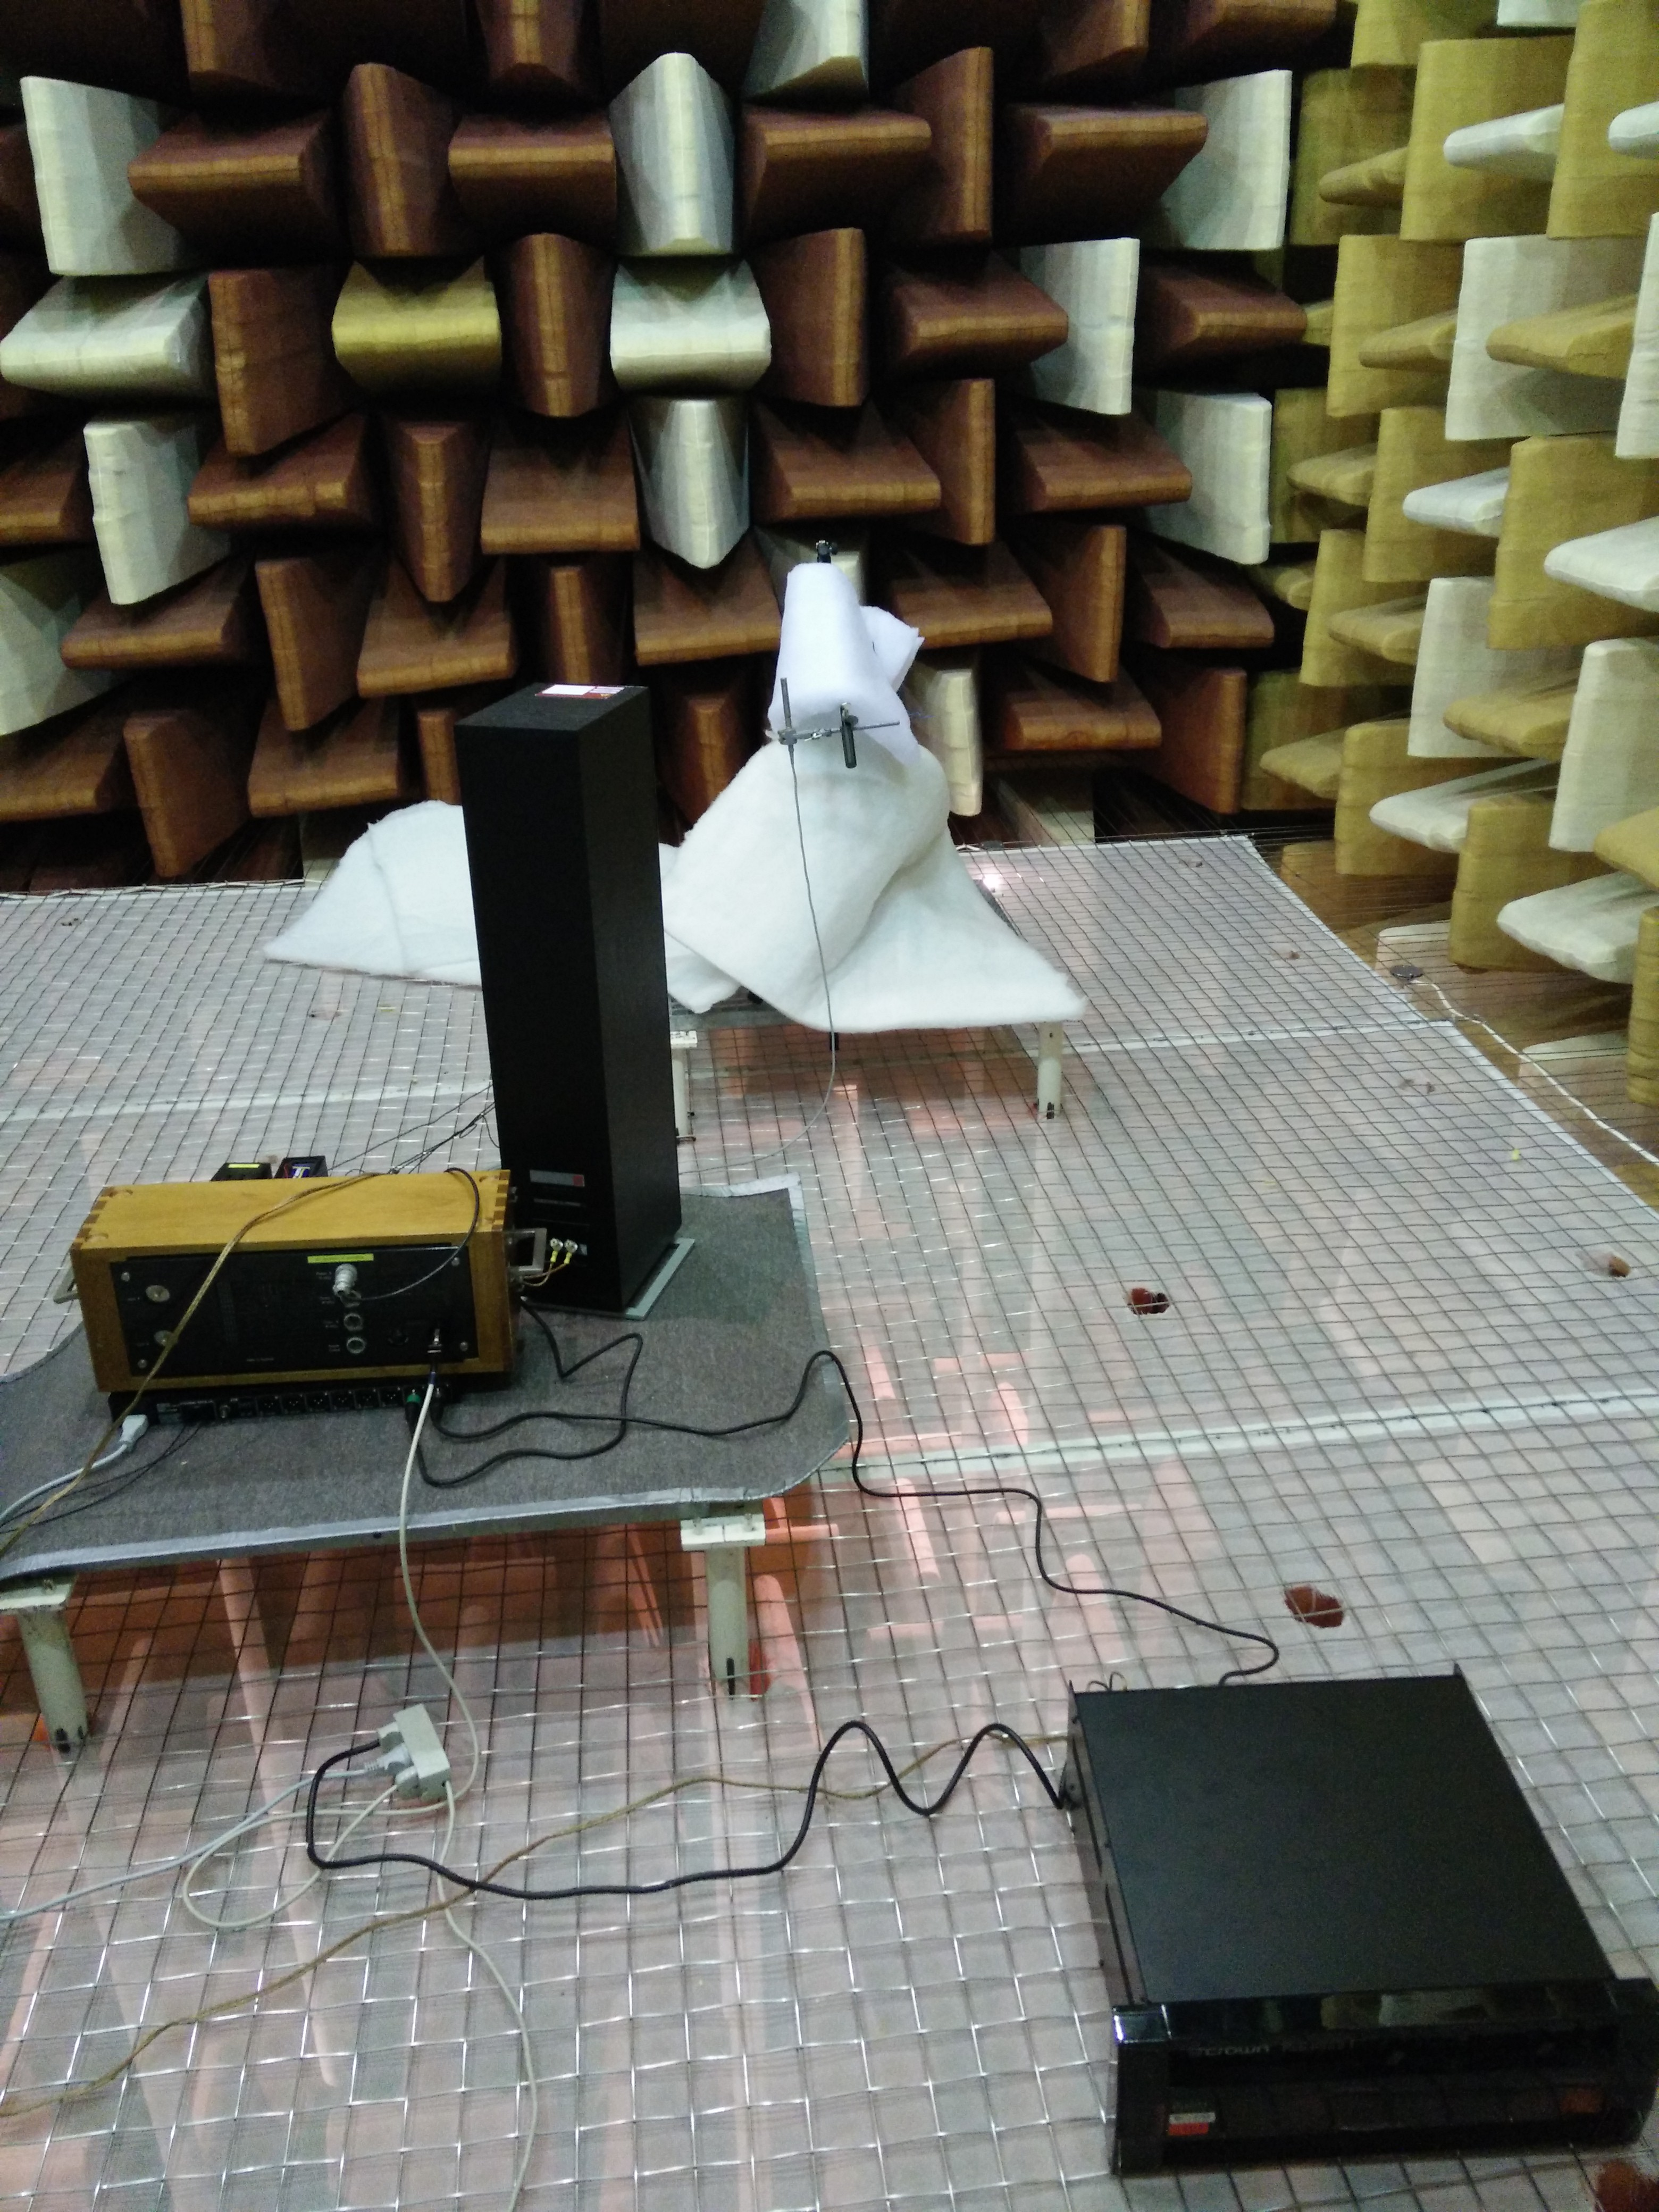
\includegraphics[width=1\textwidth]{figures/Test_setup_behind.jpg}
	\caption{Test setup (behind)}
	\label{fig:test_setup_behind_R}
\end{subfigure}
\hspace{6mm} 
\begin{subfigure}[t]{0.47\textwidth}
	\centering
	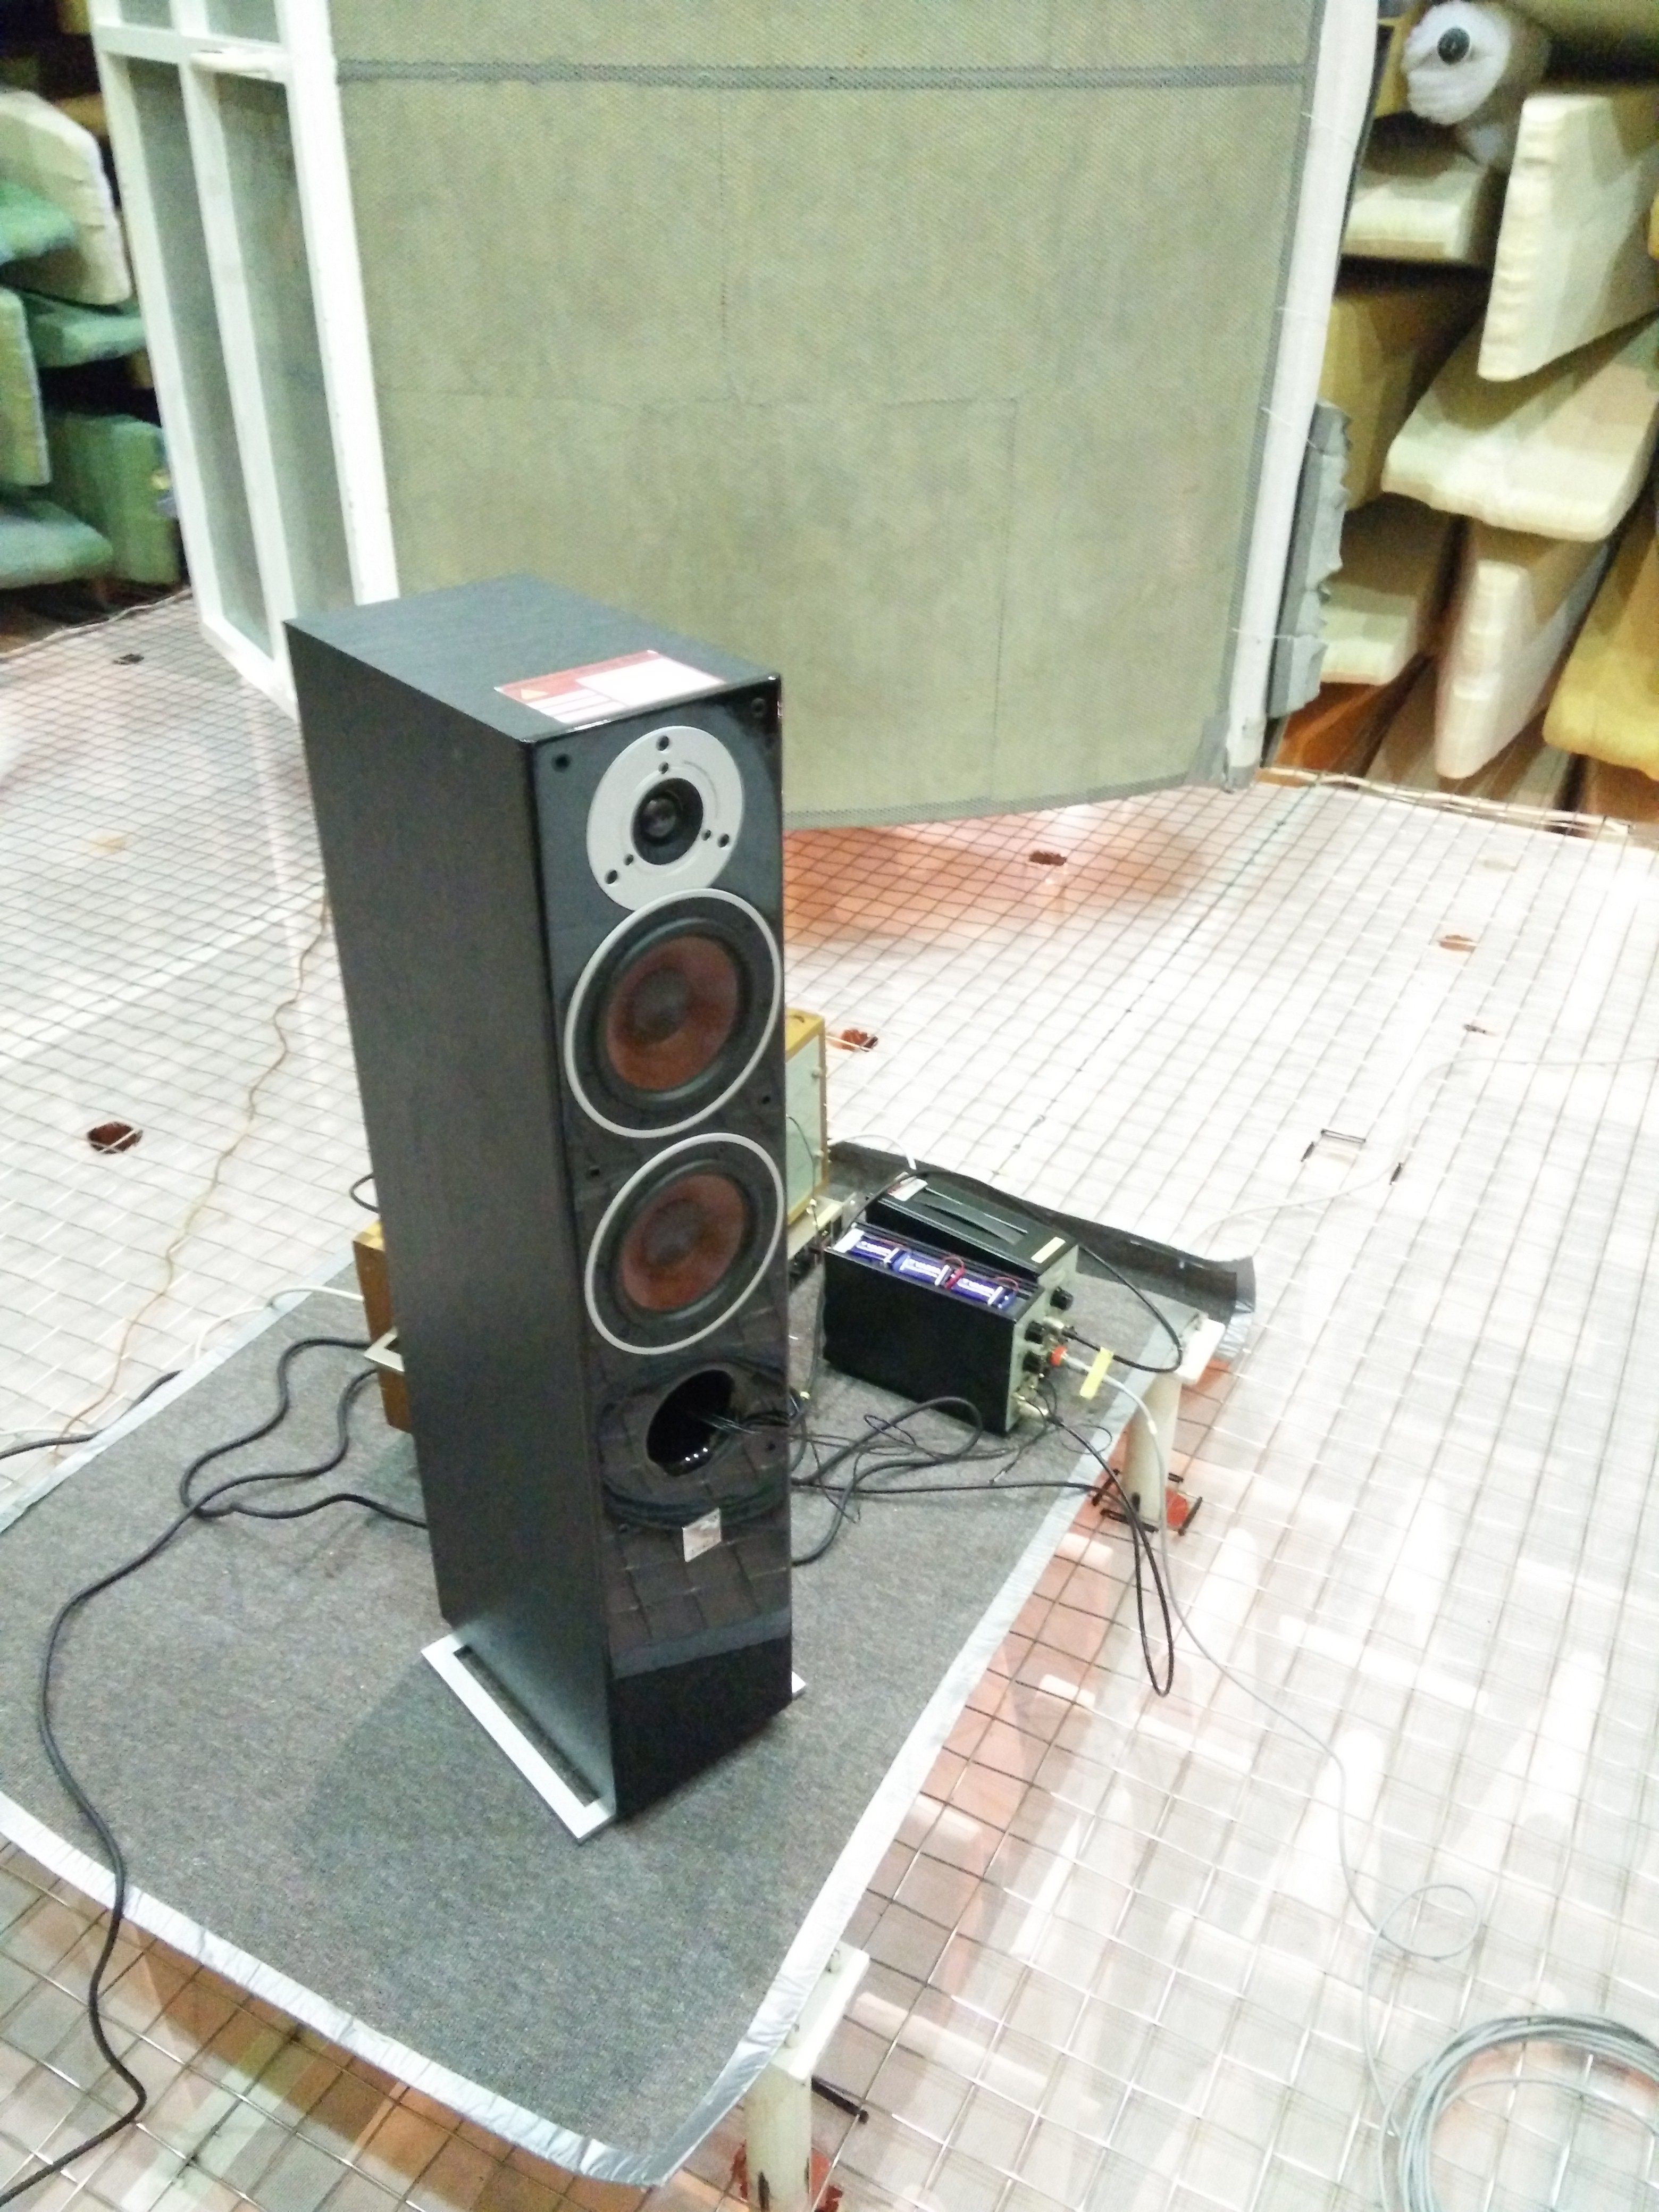
\includegraphics[width=1\textwidth]{figures/Test_setup_front.jpg}
	\caption{Test setup (front)}
	\label{fig:test_setup_front_R}
\end{subfigure}
\caption{Test setup.}
\label{fig:test_setup_R}
\end{figure}

The loudspeaker is set to play a sinesweep from the crossover frequency of the speaker which is 2400 Hz to 10 Hz. The sine sweep is then repeated from the lowest volume setting of an power amplifier until the loudspeaker breaks. This resulted in 20 sine sweep measurements from all three sensors which can be seen in the full test jounal in \autoref{app:journal_speaker_test}.    


\section{Analysis of the DALI Zensor AX 5 measurements}

In this section an analysis of the data extracted from the test DALI Zensor 5 AX will be presented. The purpose of this analysis is to examine if it possible to tell the current performance of the loudspeaker from the accelerometer placed on the loudspeaker. There are many different approaches in analysing the measured data, and the extent of the analysis will be analysing the frequency response of the loudspeaker vibration, harmonic distortion, and detection of the coil hitting the back plate of the driver. The structure of the following part of this section will be:

\begin{itemize}
\item Presentation of the measured data.
\item Frequency response of the measured data.
\item Harmonic distortion measured by the microphone and accelerometers.
\item Back plate hit detection.
\end{itemize}

Before analysing the measured the measured data will be presented.

\section{Introduction to Measured Data}

As previously stated there are in total 20 datasets each containing four measurements, namely the vibrations from the enclosure and driver, the sound pressure from the microphone, and lastly a reference signal to synchronize all data. The amount of data is therefore large and only relevant datasets will be presented. The remaining data are available on the CD. The first dataset from the test is shown in \autoref{fig:raw1}.

\begin{figure}[H]
\centering
\begin{subfigure}[t]{0.335\textwidth}
	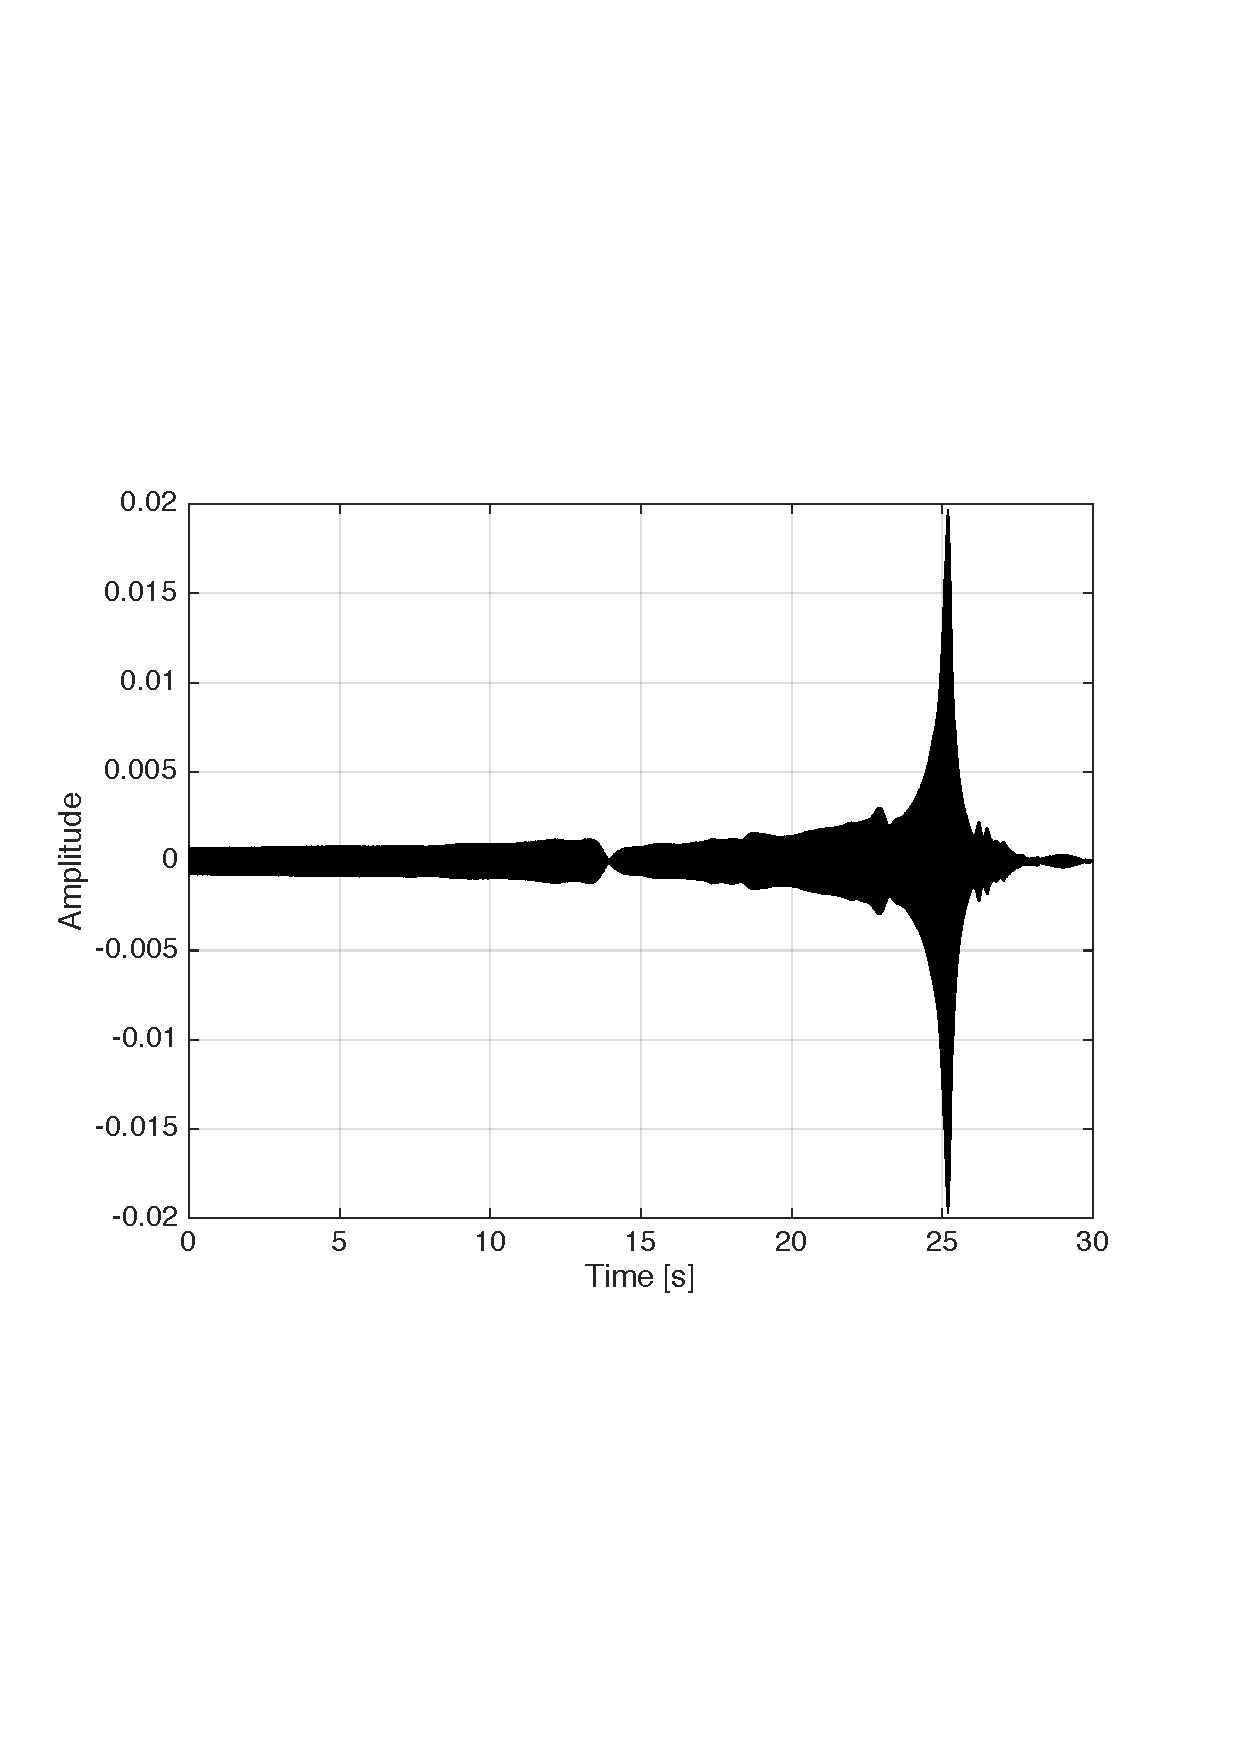
\includegraphics[width=1\textwidth]{figures/raw_driver1.pdf}
	\caption{Vibration from driver.}
	\label{fig:raw_driver1}
\end{subfigure}
\begin{subfigure}[t]{0.3\textwidth}
	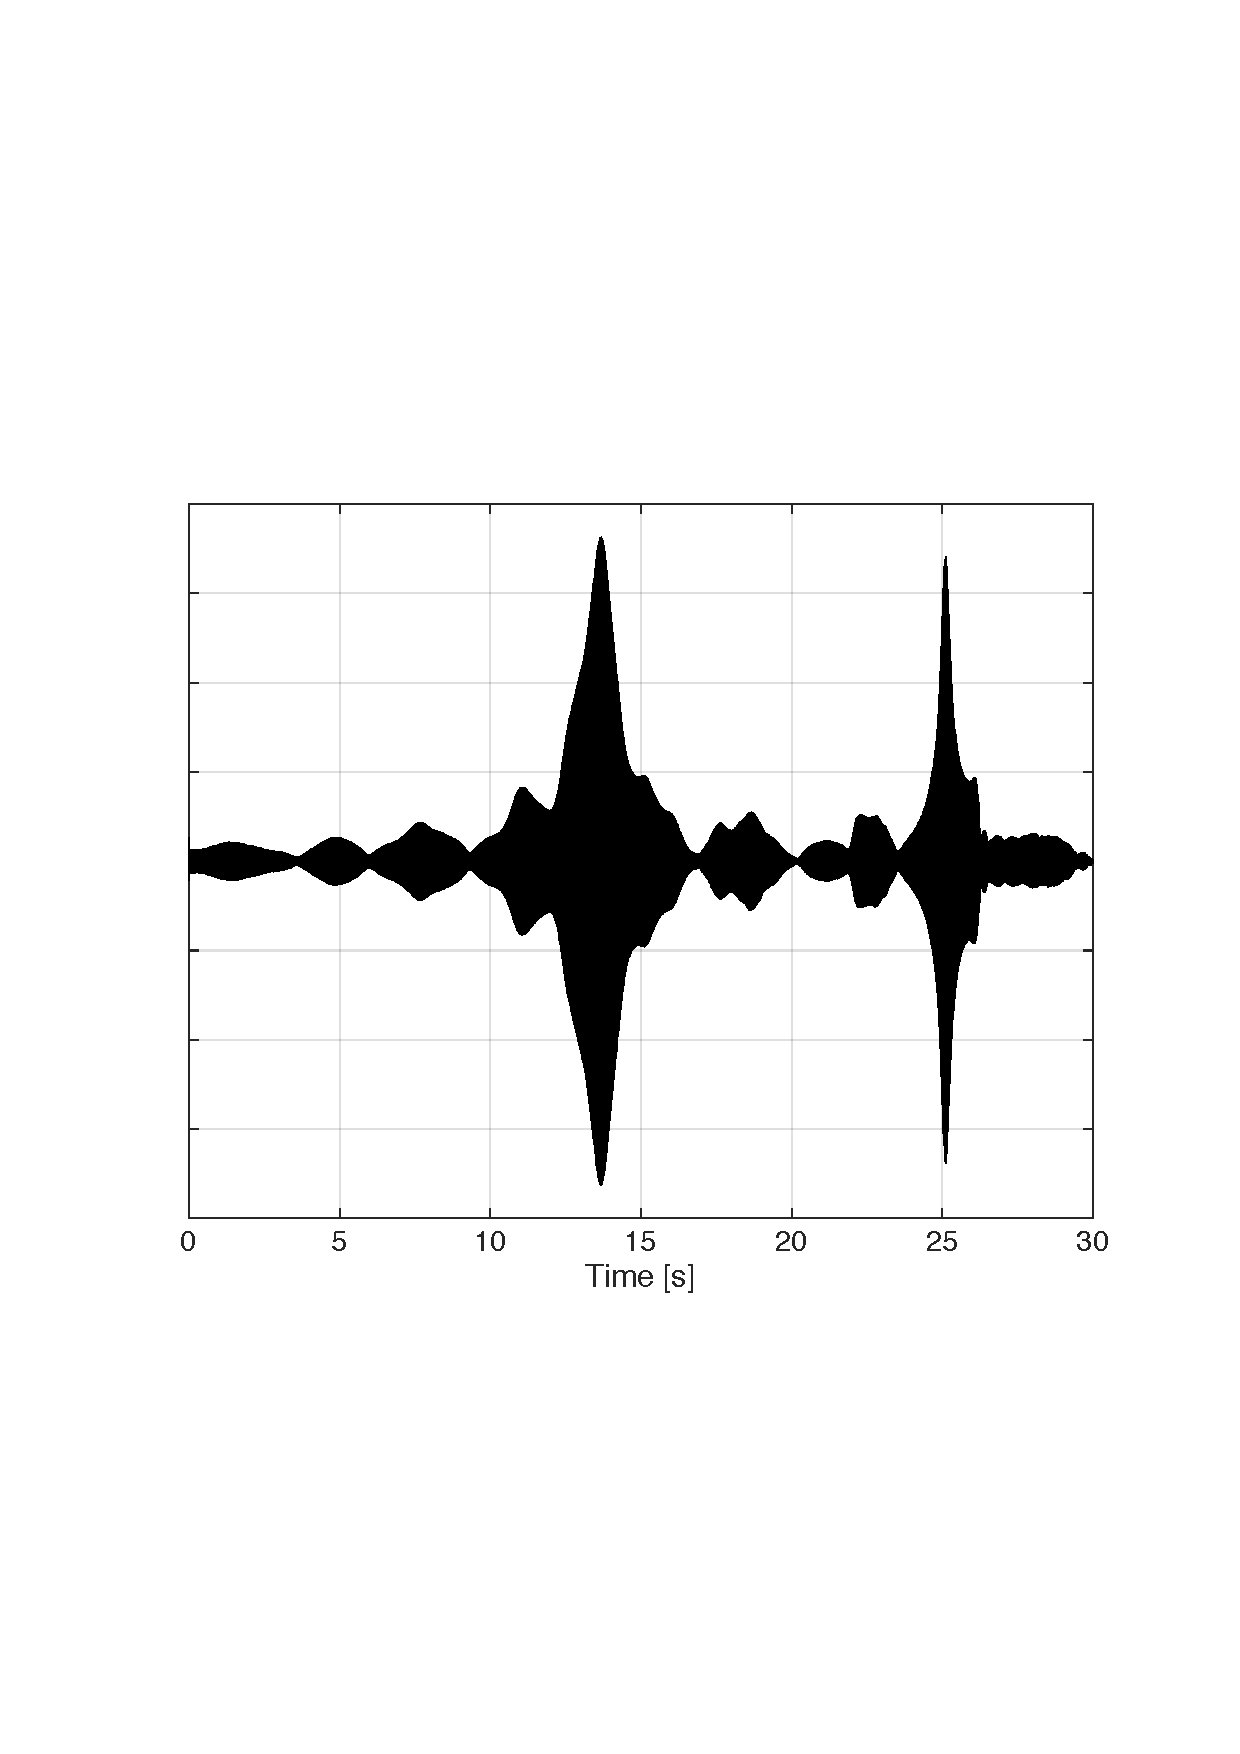
\includegraphics[width=1\textwidth]{figures/raw_enclosure1.pdf}
	\caption{Vibration from enclosure.}
	\label{fig:raw_enclosure1}
\end{subfigure}
\begin{subfigure}[t]{0.3\textwidth}
	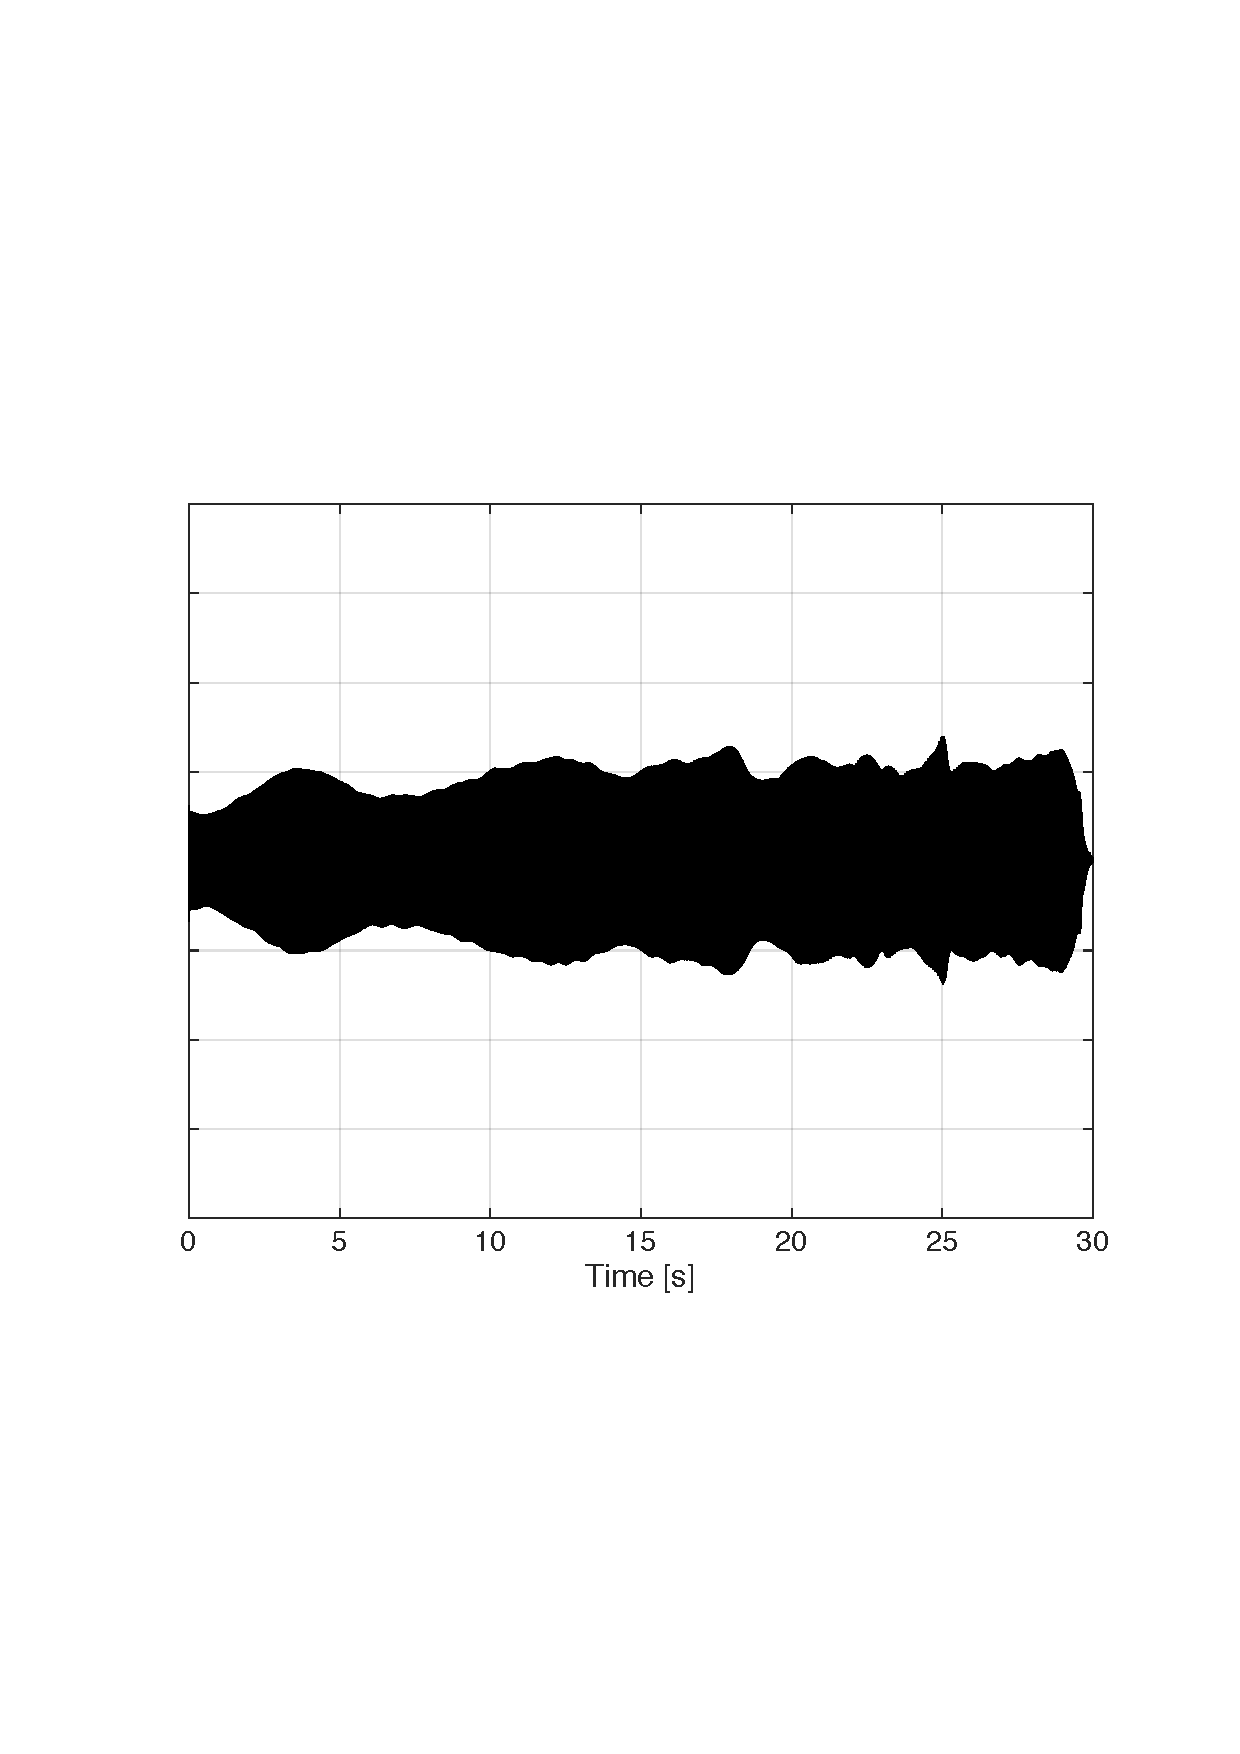
\includegraphics[width=1\textwidth]{figures/raw_microphone1.pdf}
	\caption{Sound pressure from microphone.}
	\label{fig:raw_microphone1}
\end{subfigure}
\caption{The measured data of (a) the vibration on the driver, (b) the vibration on the enclosure, and (c) the sound pressure from the microphone. Dataset 1.}
\label{fig:raw1}
\end{figure} 

Looking at the first dataset reveals that there are mechanical issues with the loudspeaker. In \autoref{fig:raw_driver1} there is a strong indication of a resonance frequency at 25 seconds with a peak amplitude on approximately 0.02. A similar observation can be found in \autoref{fig:raw_enclosure1} which shows the vibration measured by the accelerometer placed on the enclosure where a resonance frequency appears after 25 seconds. Another mechanical resonance frequency can be found located after 14 seconds for the enclosure. The sound pressure level measured by the microphone is in contrast fairly linear compared to the measured vibrations. Dataset 10 is shown in \autoref{fig:raw10} where the gain is increased by 10 dB.

\begin{figure}[H]
\centering
\begin{subfigure}[t]{0.335\textwidth}
	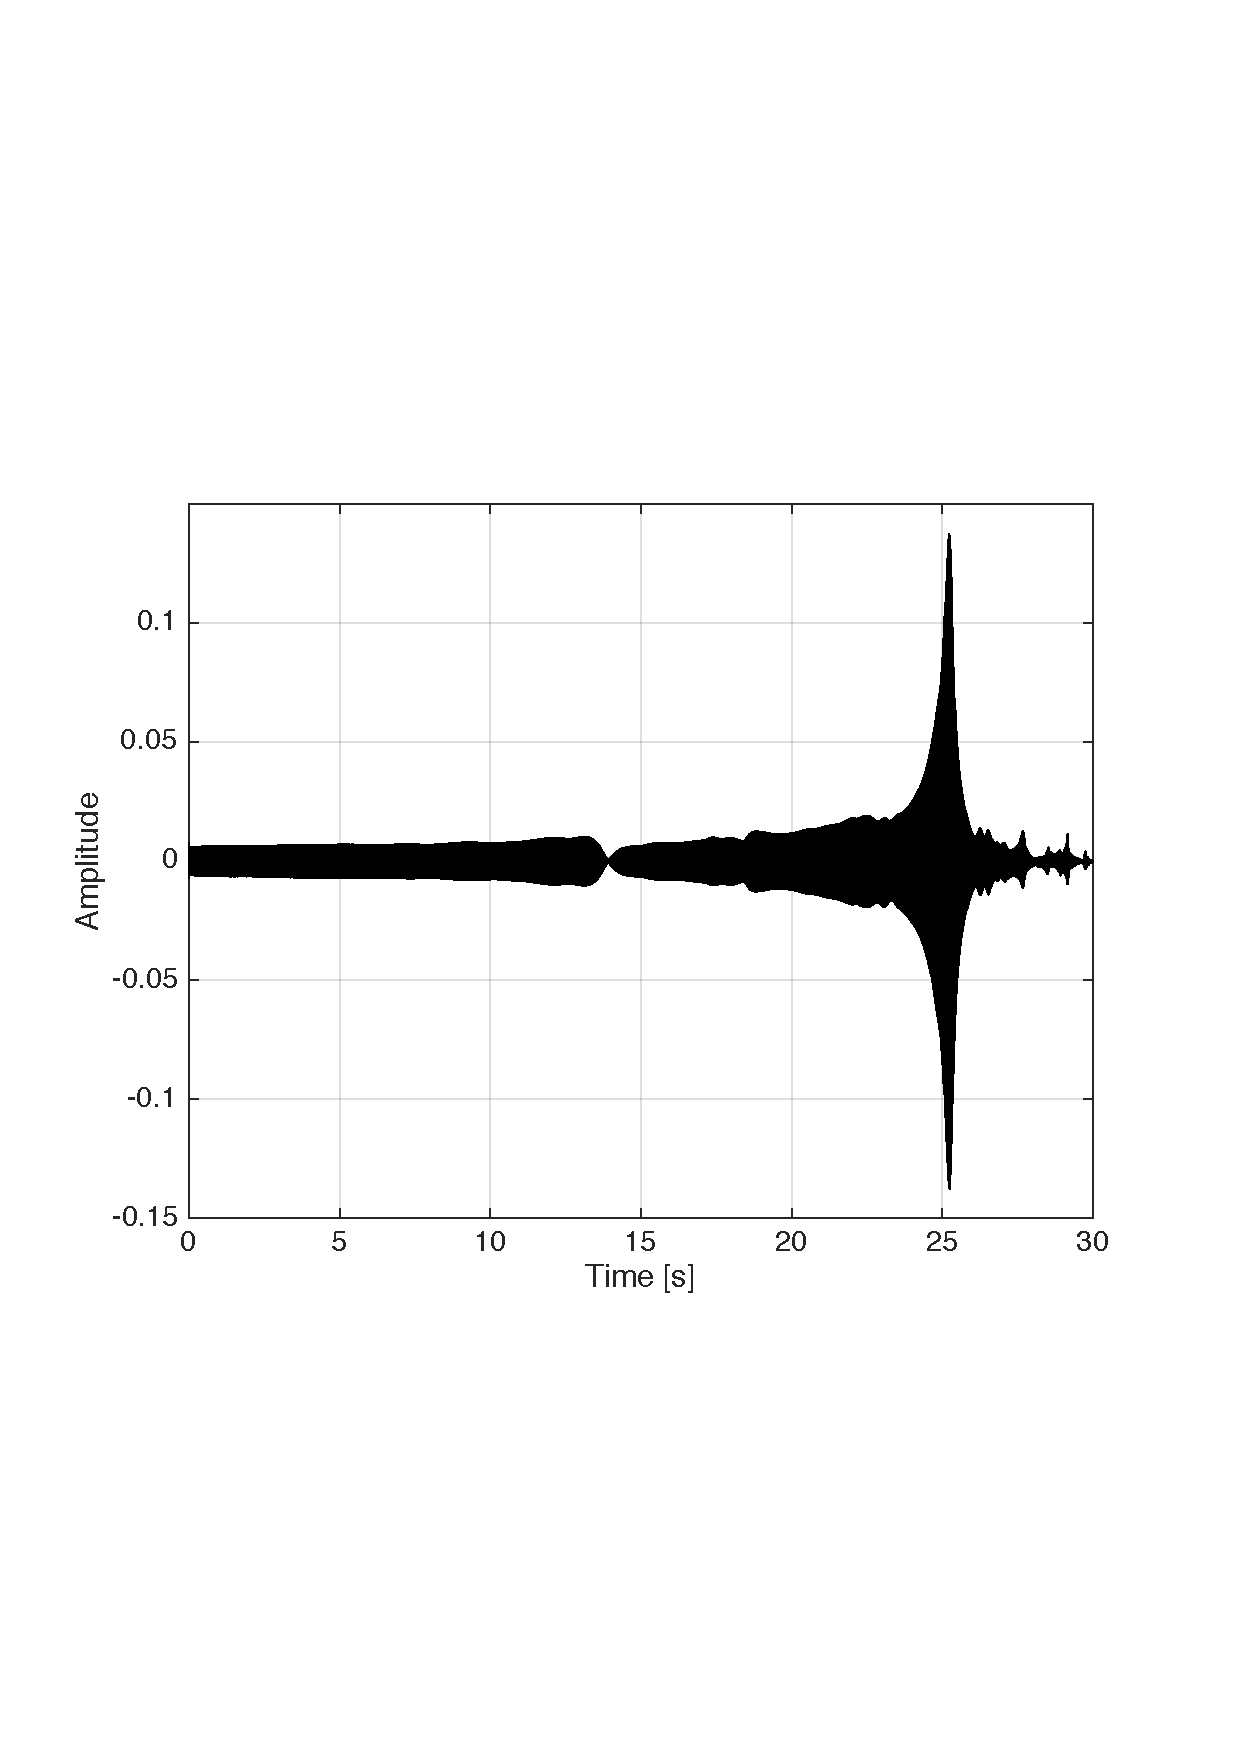
\includegraphics[width=1\textwidth]{figures/raw_driver10.pdf}
	\caption{Vibration from driver.}
	\label{fig:raw_driver10}
\end{subfigure}
\begin{subfigure}[t]{0.3\textwidth}
	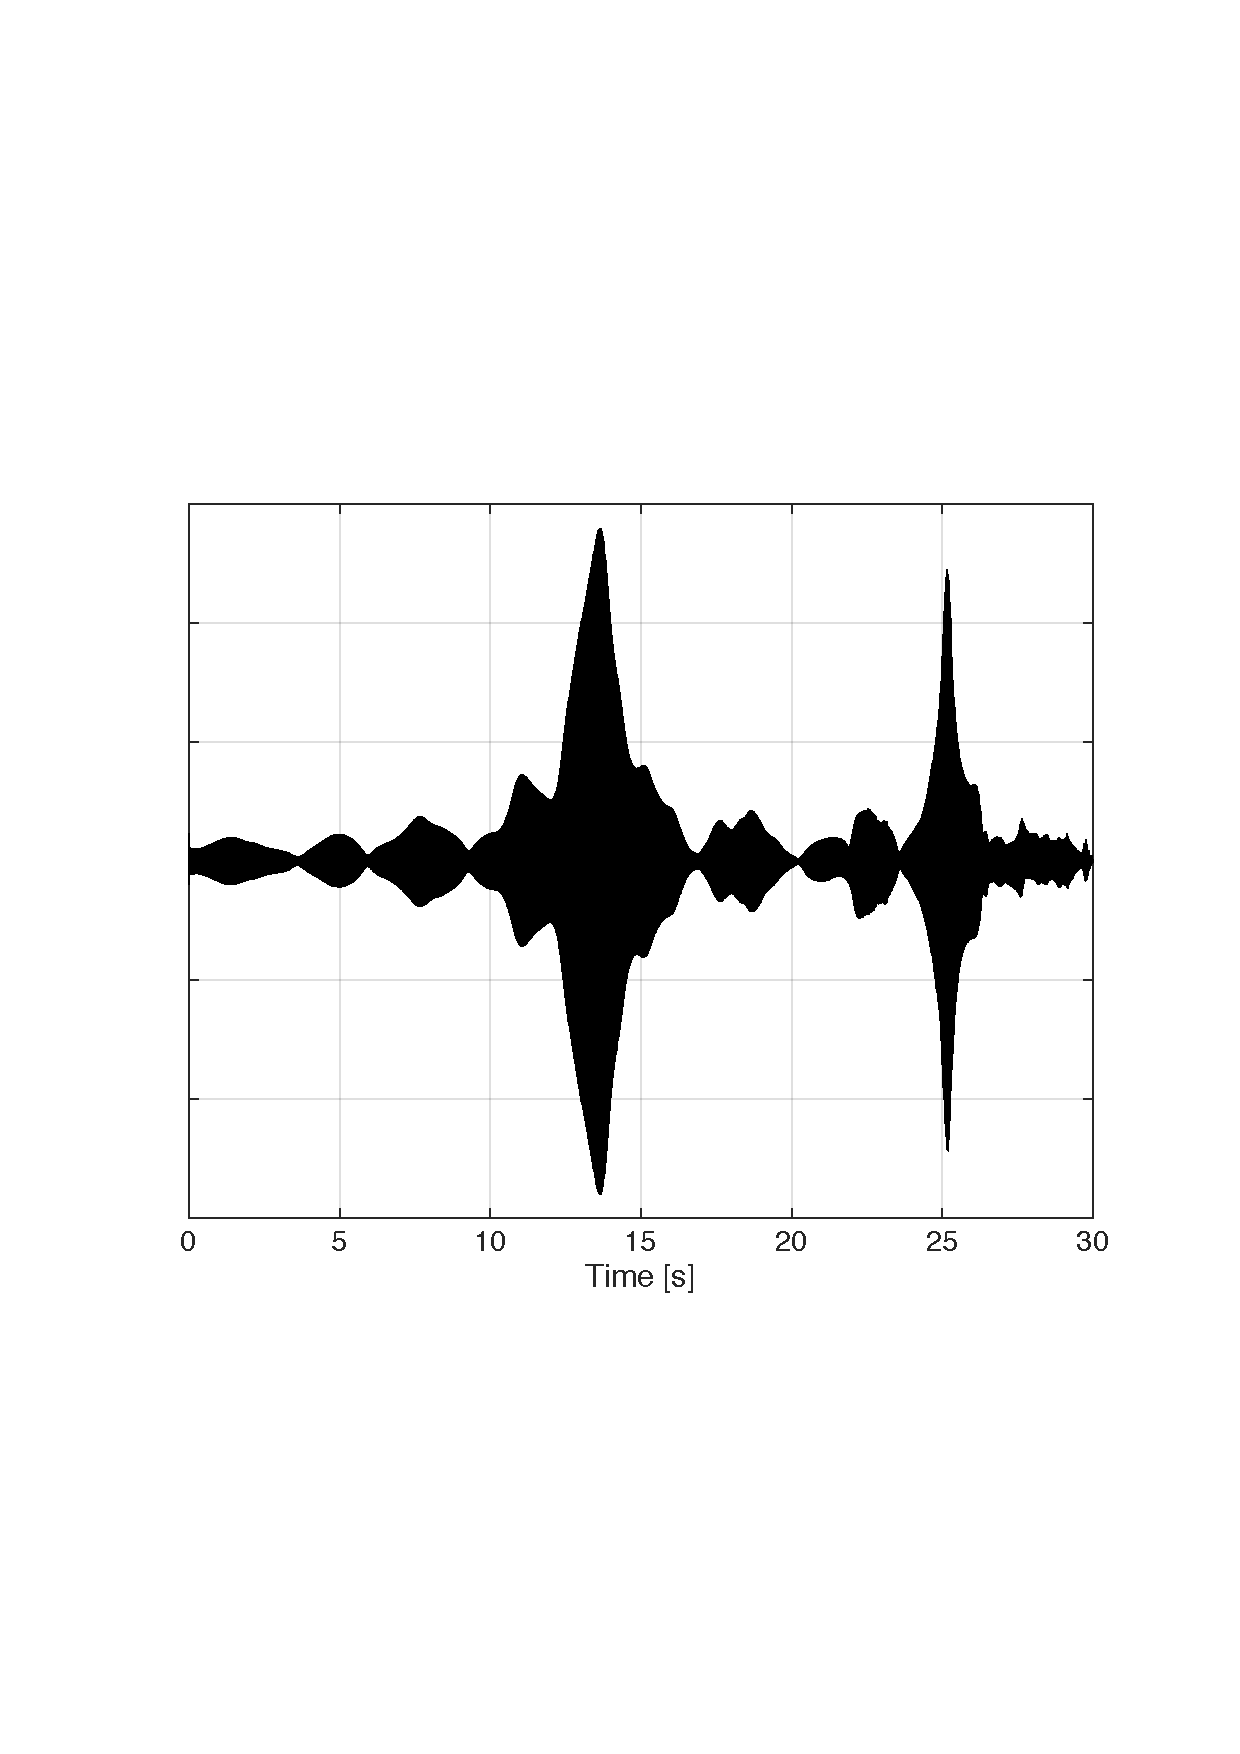
\includegraphics[width=1\textwidth]{figures/raw_enclosure10.pdf}
	\caption{Vibration from enclosure.}
	\label{fig:raw_enclosure10}
\end{subfigure}
\begin{subfigure}[t]{0.3\textwidth}
	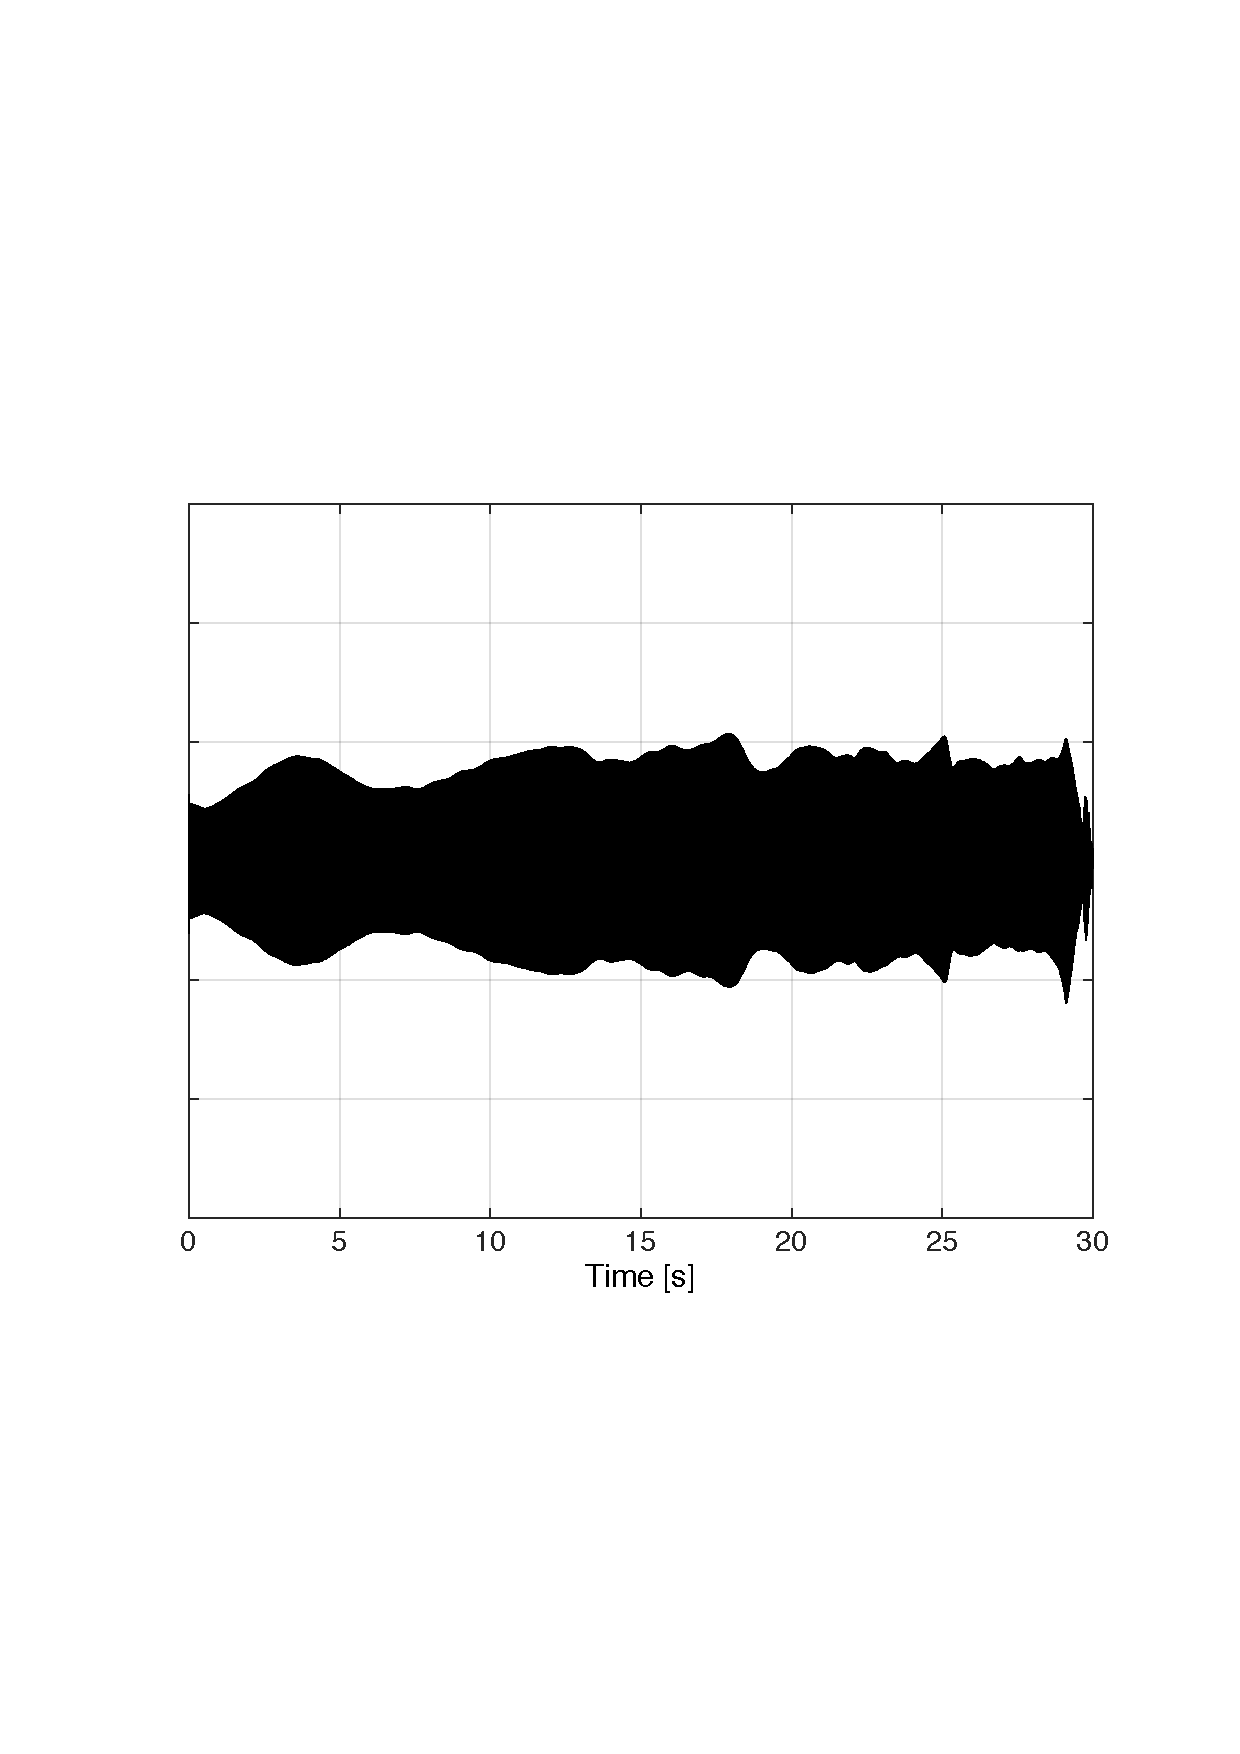
\includegraphics[width=1\textwidth]{figures/raw_microphone10.pdf}
	\caption{Sound pressure from microphone.}
	\label{fig:raw_microphone10}
\end{subfigure}
\caption{The measured data of (a) the vibration on the driver, (b) the vibration on the enclosure, and (c) the sound pressure from the microphone. Dataset 10.}
\label{fig:raw10}
\end{figure} 

The measurements from dataset 10 is very similar to the measurements seen in dataset 1. Since no particular change is happening between dataset 1 to 10 it is assumed that the performance of the loudspeaker remains good. A further analysis of the performance speaker will be done in the analysis of the harmonic distortion section to examine the amount of harmonic distortion present. Dataset 14 is shown in \autoref{fig:raw14}. 

\begin{figure}[H]
\centering
\begin{subfigure}[t]{0.335\textwidth}
	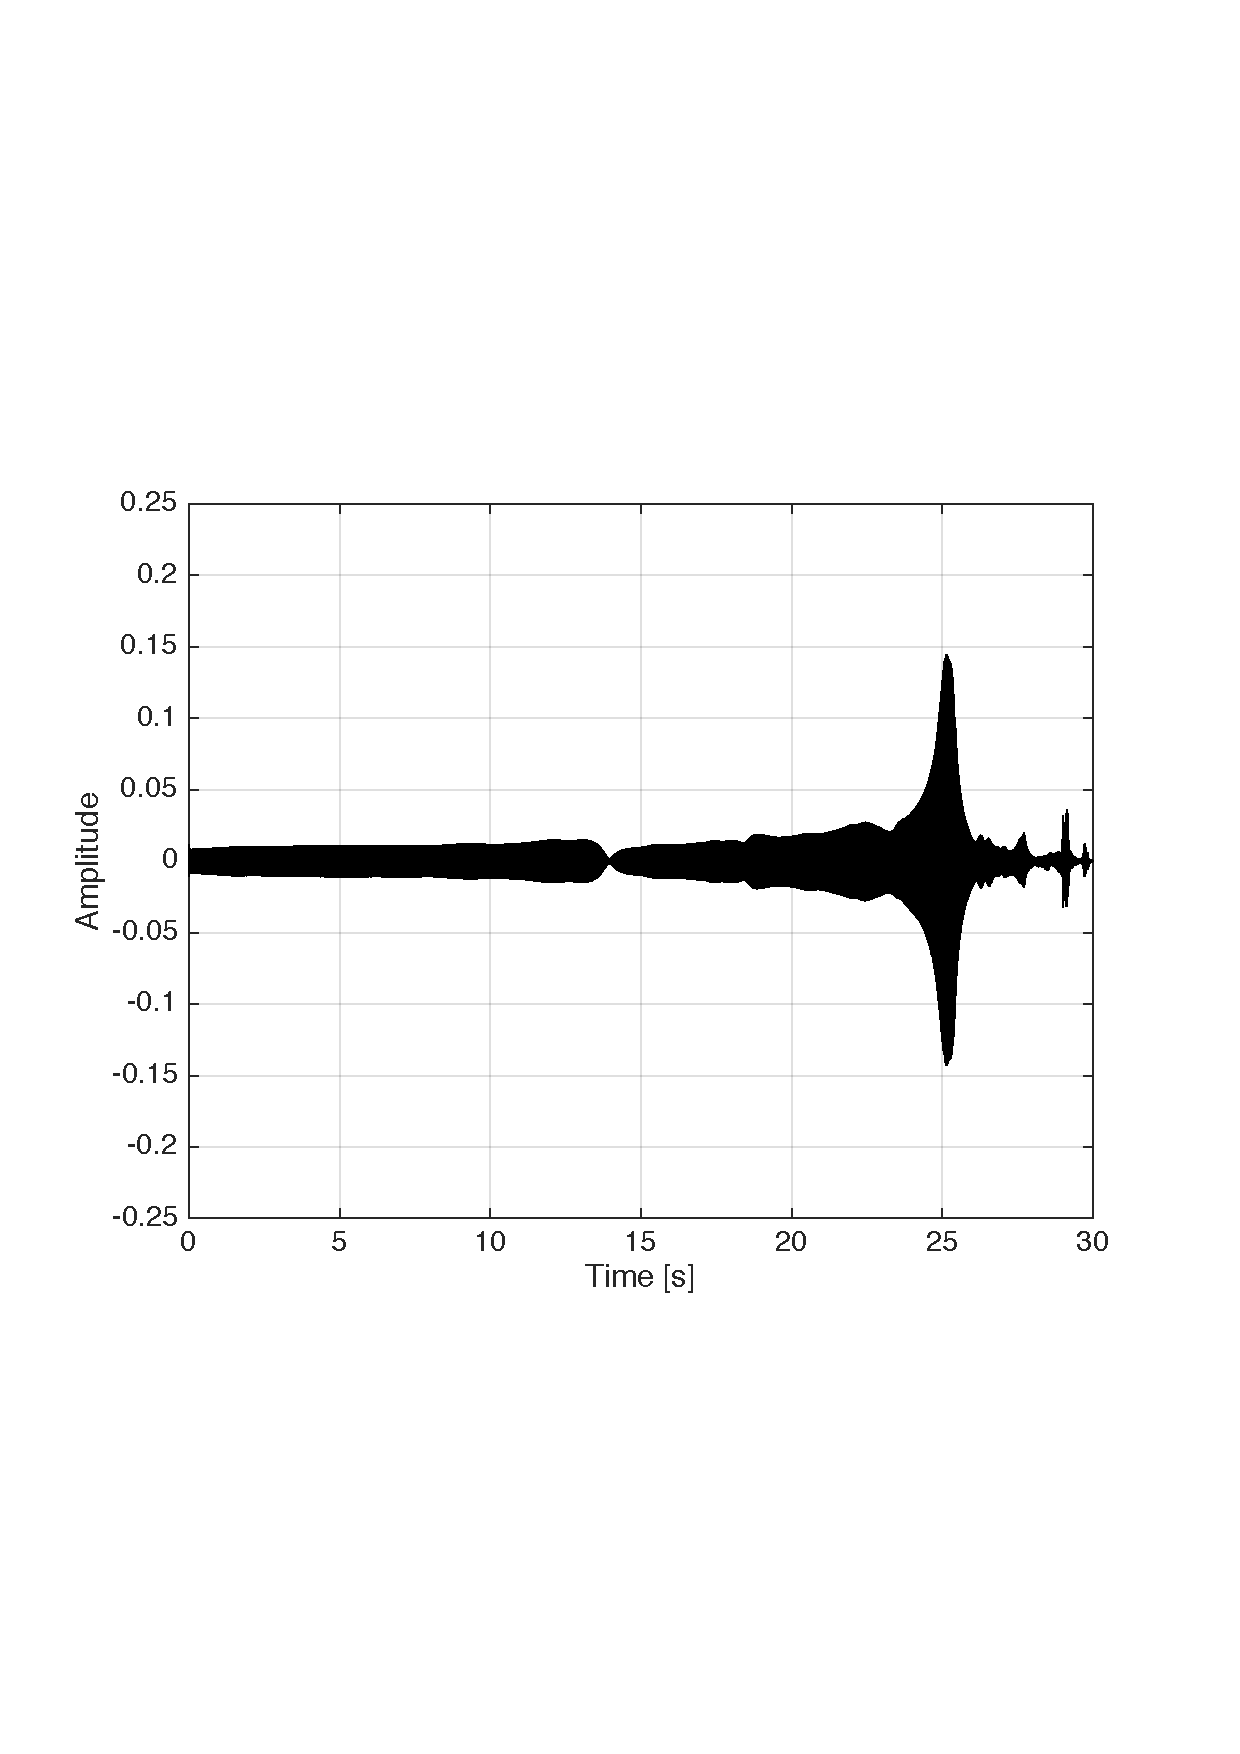
\includegraphics[width=1\textwidth]{figures/raw_driver14.pdf}
	\caption{Vibration from driver.}
	\label{fig:raw_driver14}
\end{subfigure}
\begin{subfigure}[t]{0.3\textwidth}
	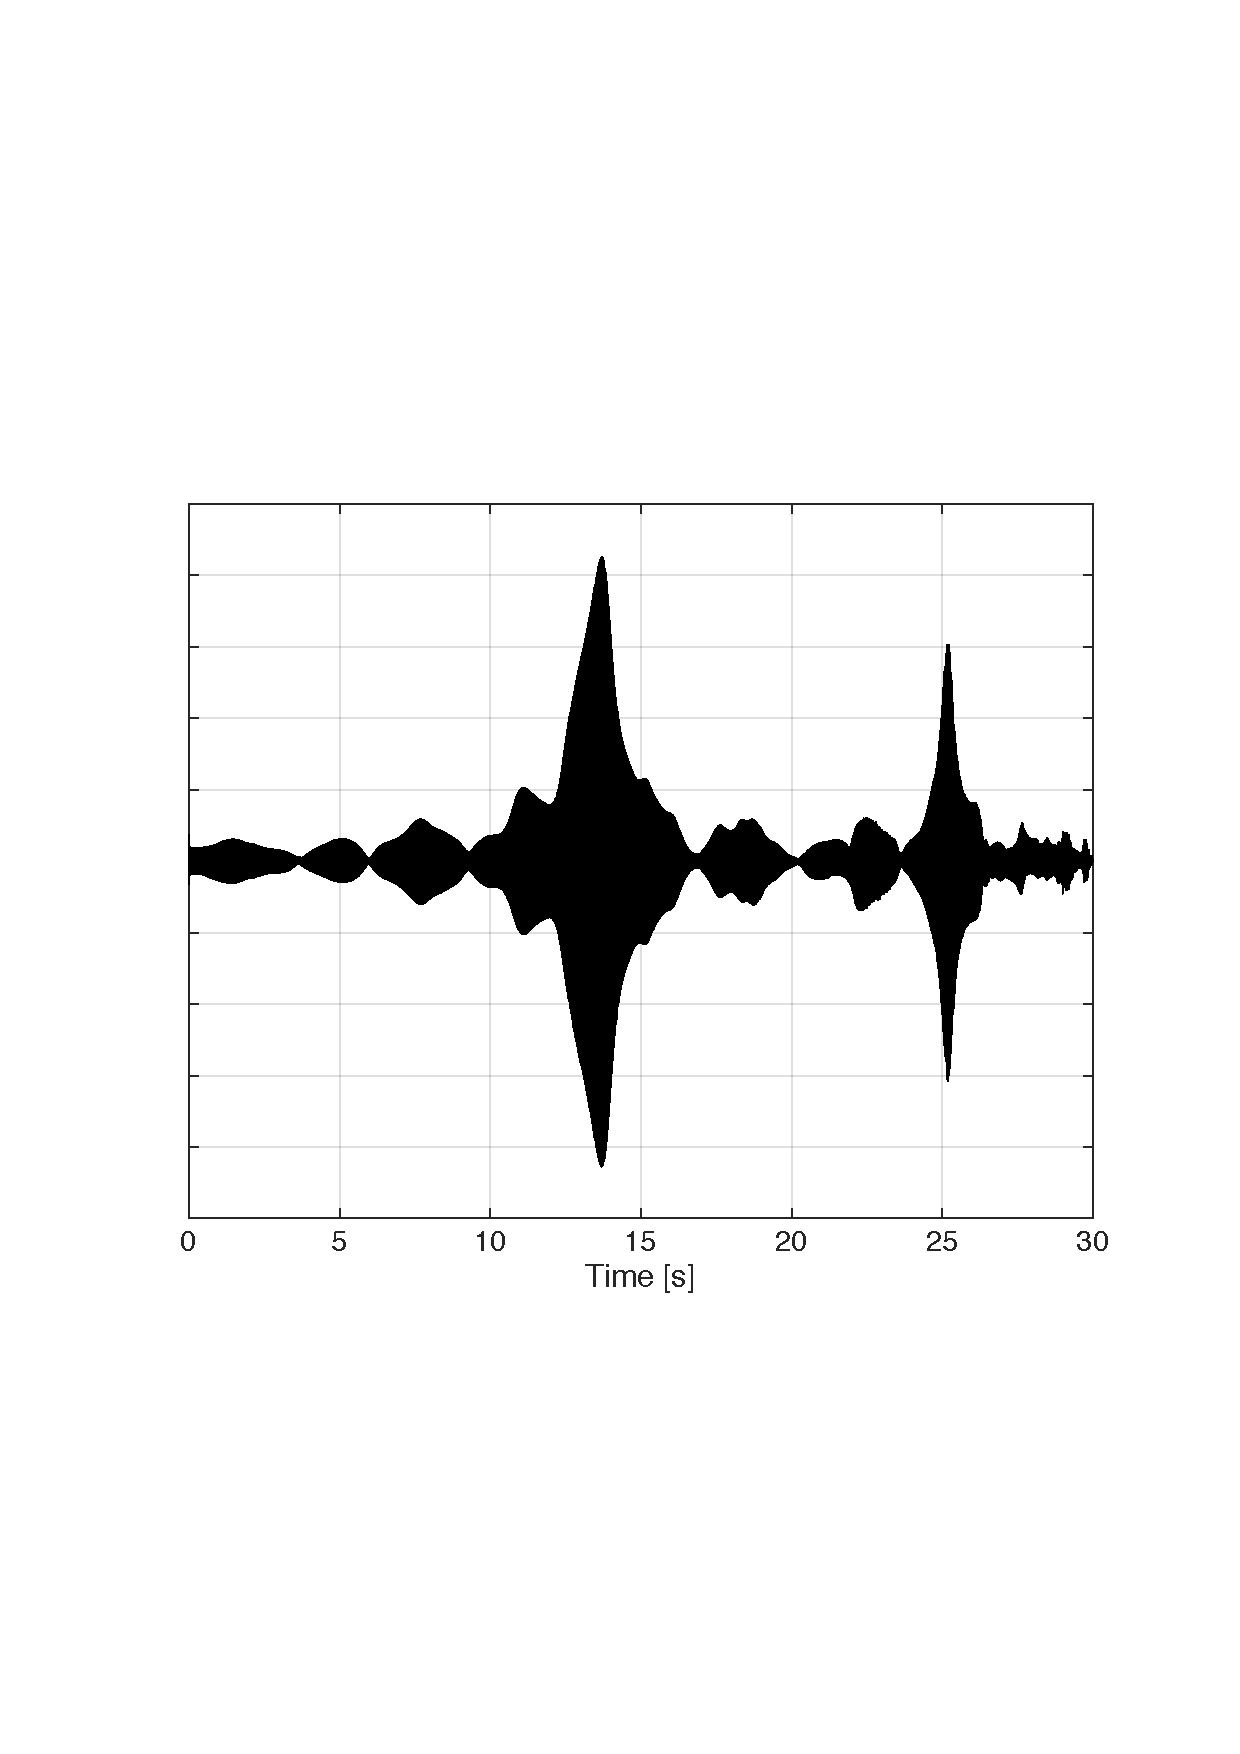
\includegraphics[width=1\textwidth]{figures/raw_enclosure14.pdf}
	\caption{Vibration from enclosure.}
	\label{fig:raw_enclosure14}
\end{subfigure}
\begin{subfigure}[t]{0.3\textwidth}
	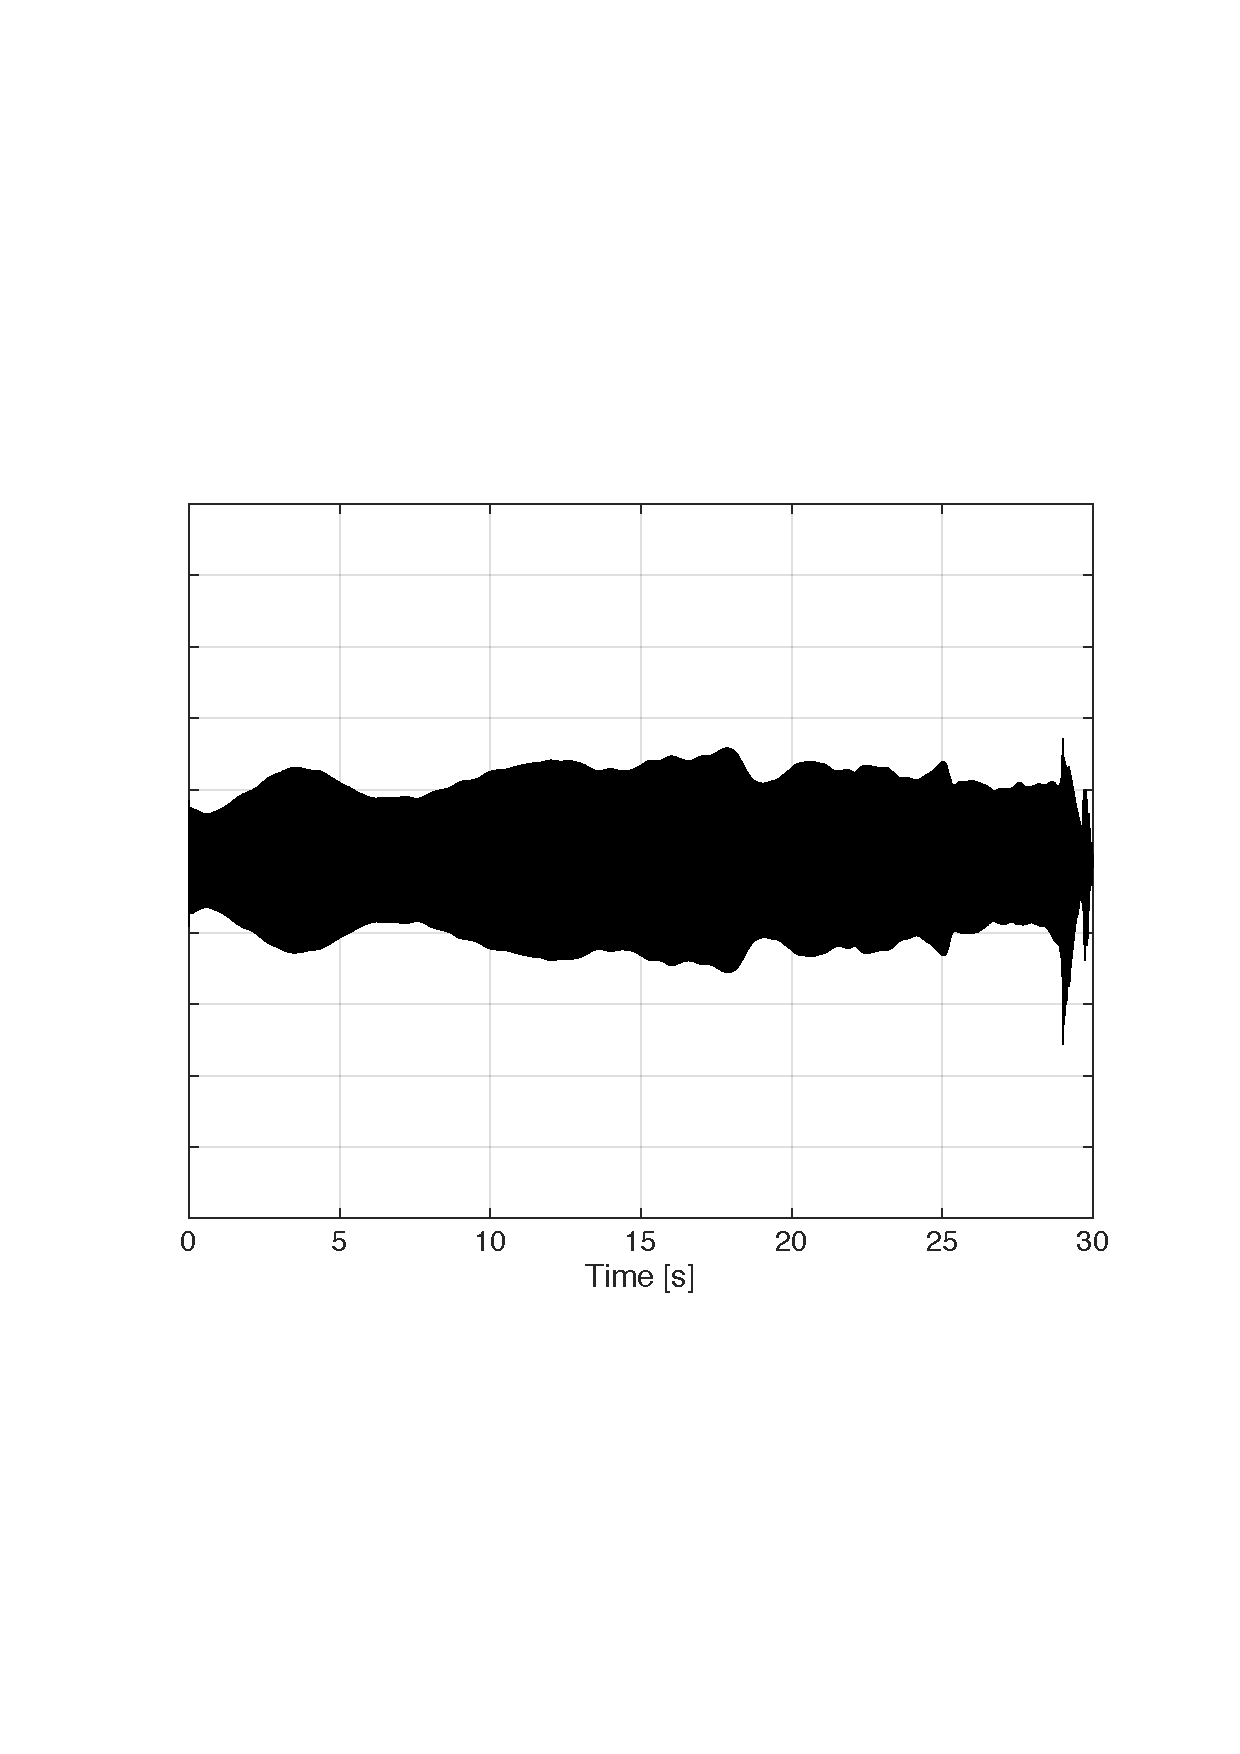
\includegraphics[width=1\textwidth]{figures/raw_microphone14.pdf}
	\caption{Sound pressure from microphone.}
	\label{fig:raw_microphone14}
\end{subfigure}
\caption{The measured data of (a) the vibration on the driver, (b) the vibration on the enclosure, and (c) the sound pressure from the microphone. Dataset 14.}
\label{fig:raw14}
\end{figure} 

While most of the measurements show the exact same characteristics as previous datasets, a slight change occurs in the end of the vibration measured on the driver in \autoref{fig:raw_driver14} and the sound pressure level in \autoref{fig:raw_microphone14}. After approximately 29 seconds a peak is observed in \autoref{fig:raw_driver14} which could indicate that the coil at that point hit the back plate of the driver. A further examination will be made in a later section. The measurements from the microphone, also show that a peak occurs at the same point, which most likely will cause the amount of harmonic distortion to increase. Dataset 19, which is the last dataset before the loudspeaker break down, is shown in \autoref{fig:raw19}.

\begin{figure}[H]
\centering
\begin{subfigure}[t]{0.335\textwidth}
	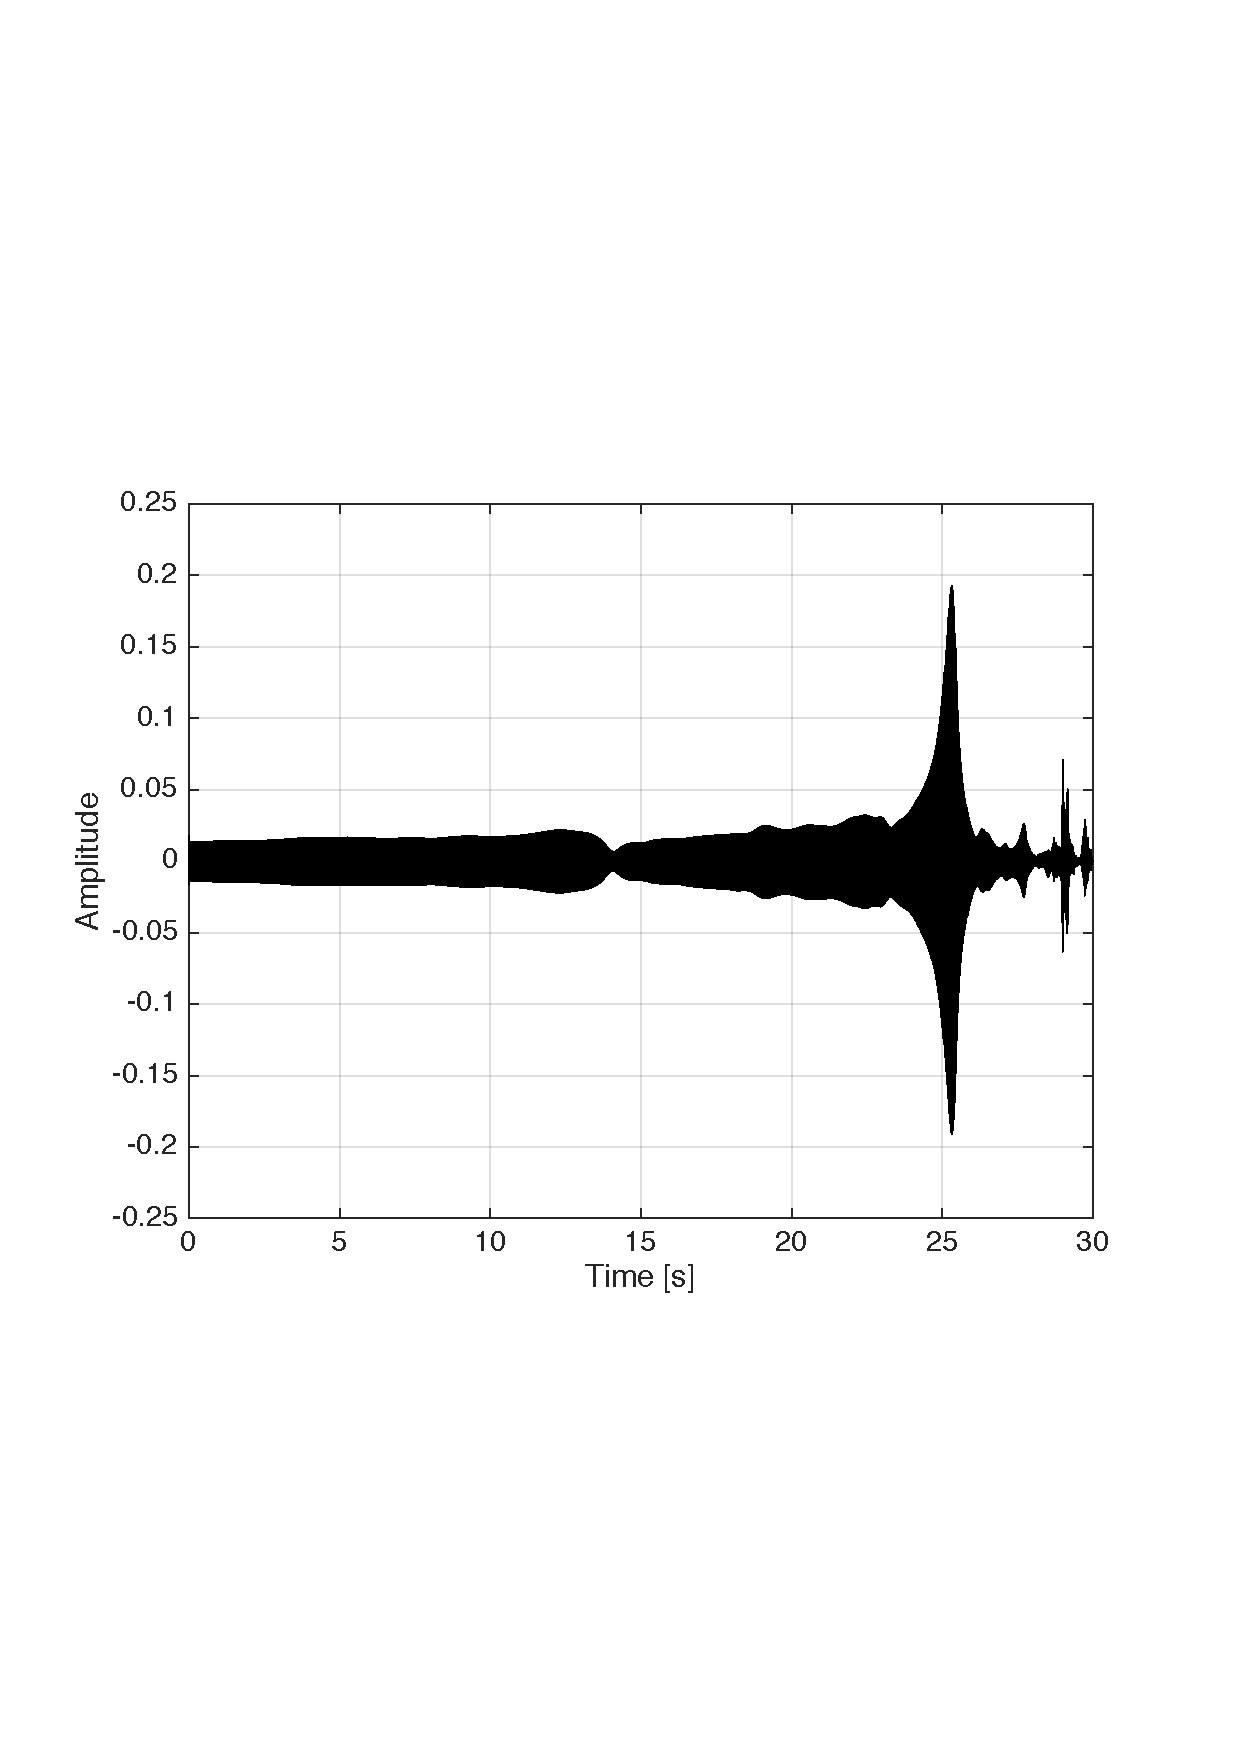
\includegraphics[width=1\textwidth]{figures/raw_driver19.pdf}
	\caption{Vibration from driver.}
	\label{fig:raw_driver19}
\end{subfigure}
\begin{subfigure}[t]{0.3\textwidth}
	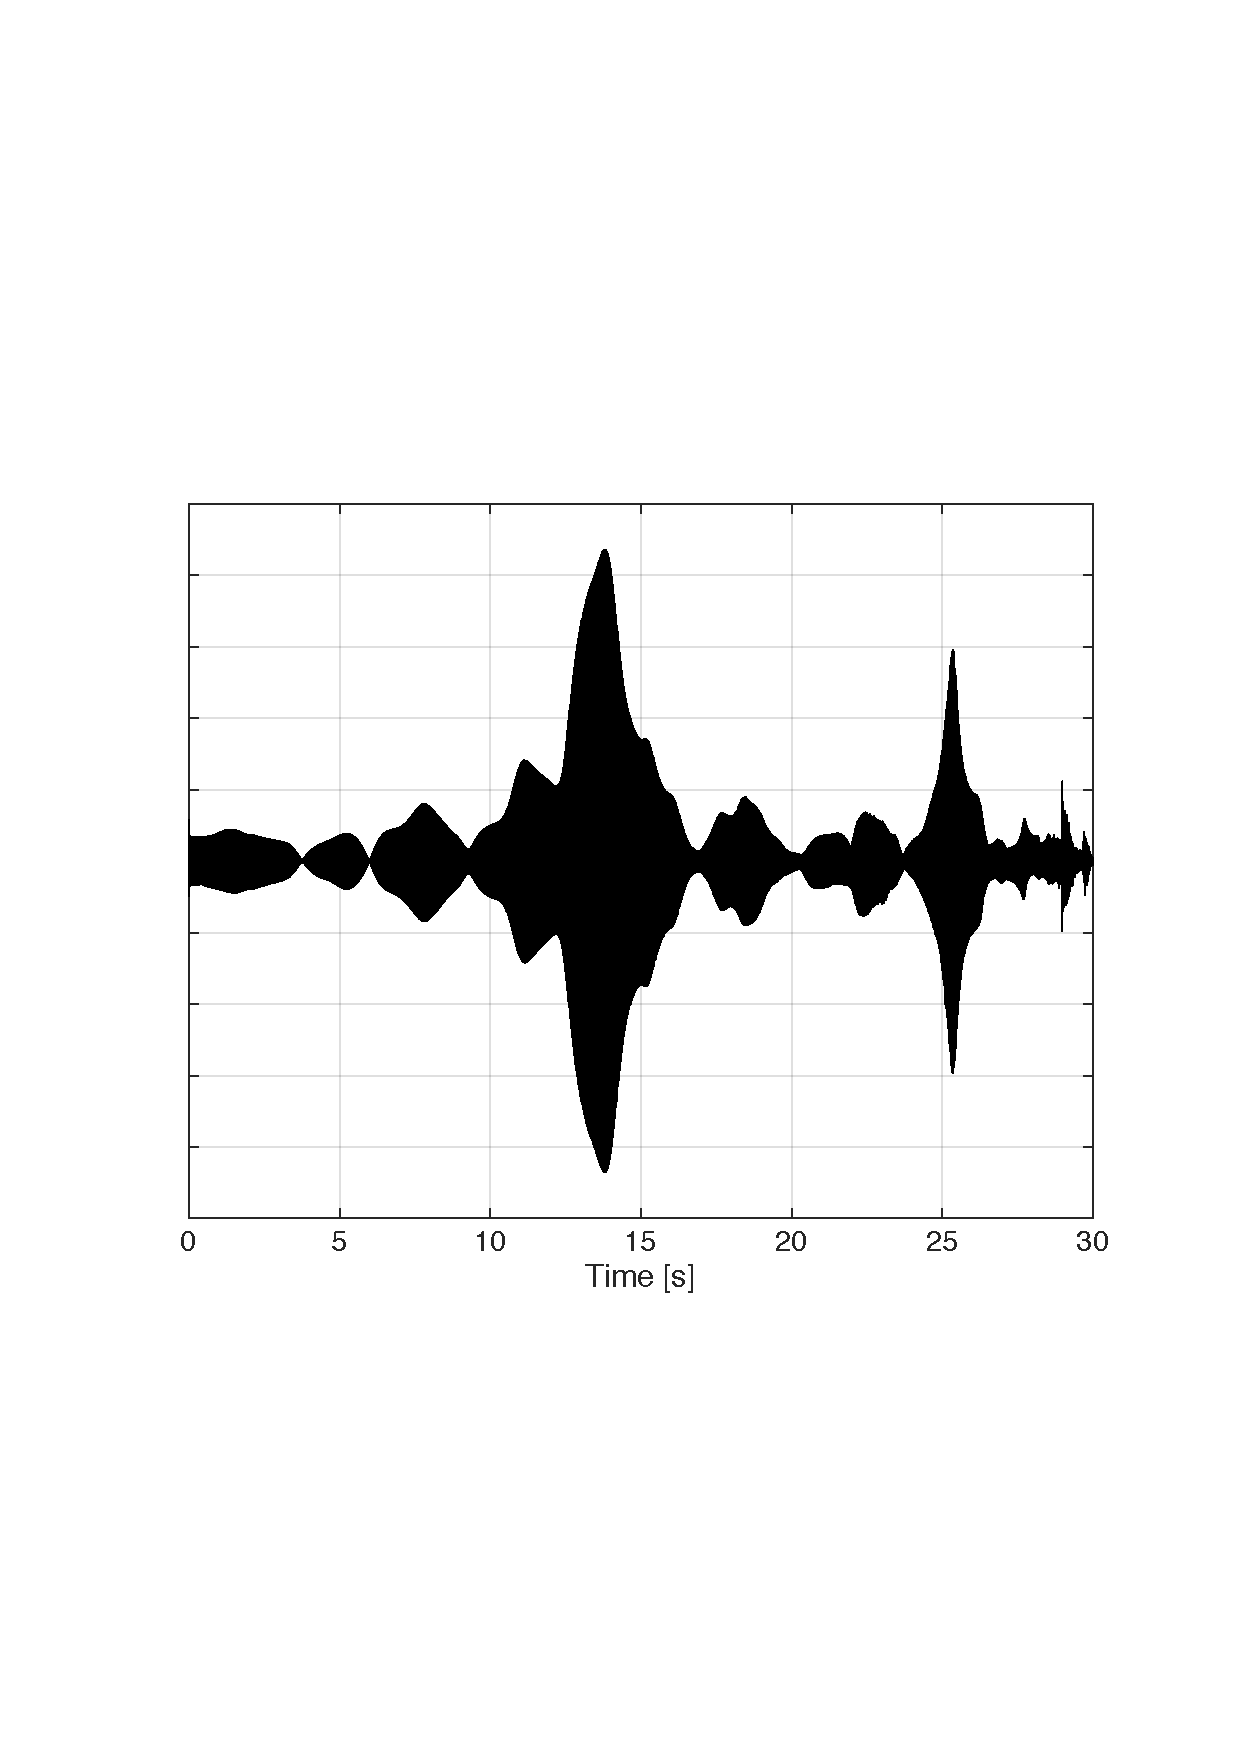
\includegraphics[width=1\textwidth]{figures/raw_enclosure19.pdf}
	\caption{Vibration from enclosure.}
	\label{fig:raw_enclosure19}
\end{subfigure}
\begin{subfigure}[t]{0.3\textwidth}
	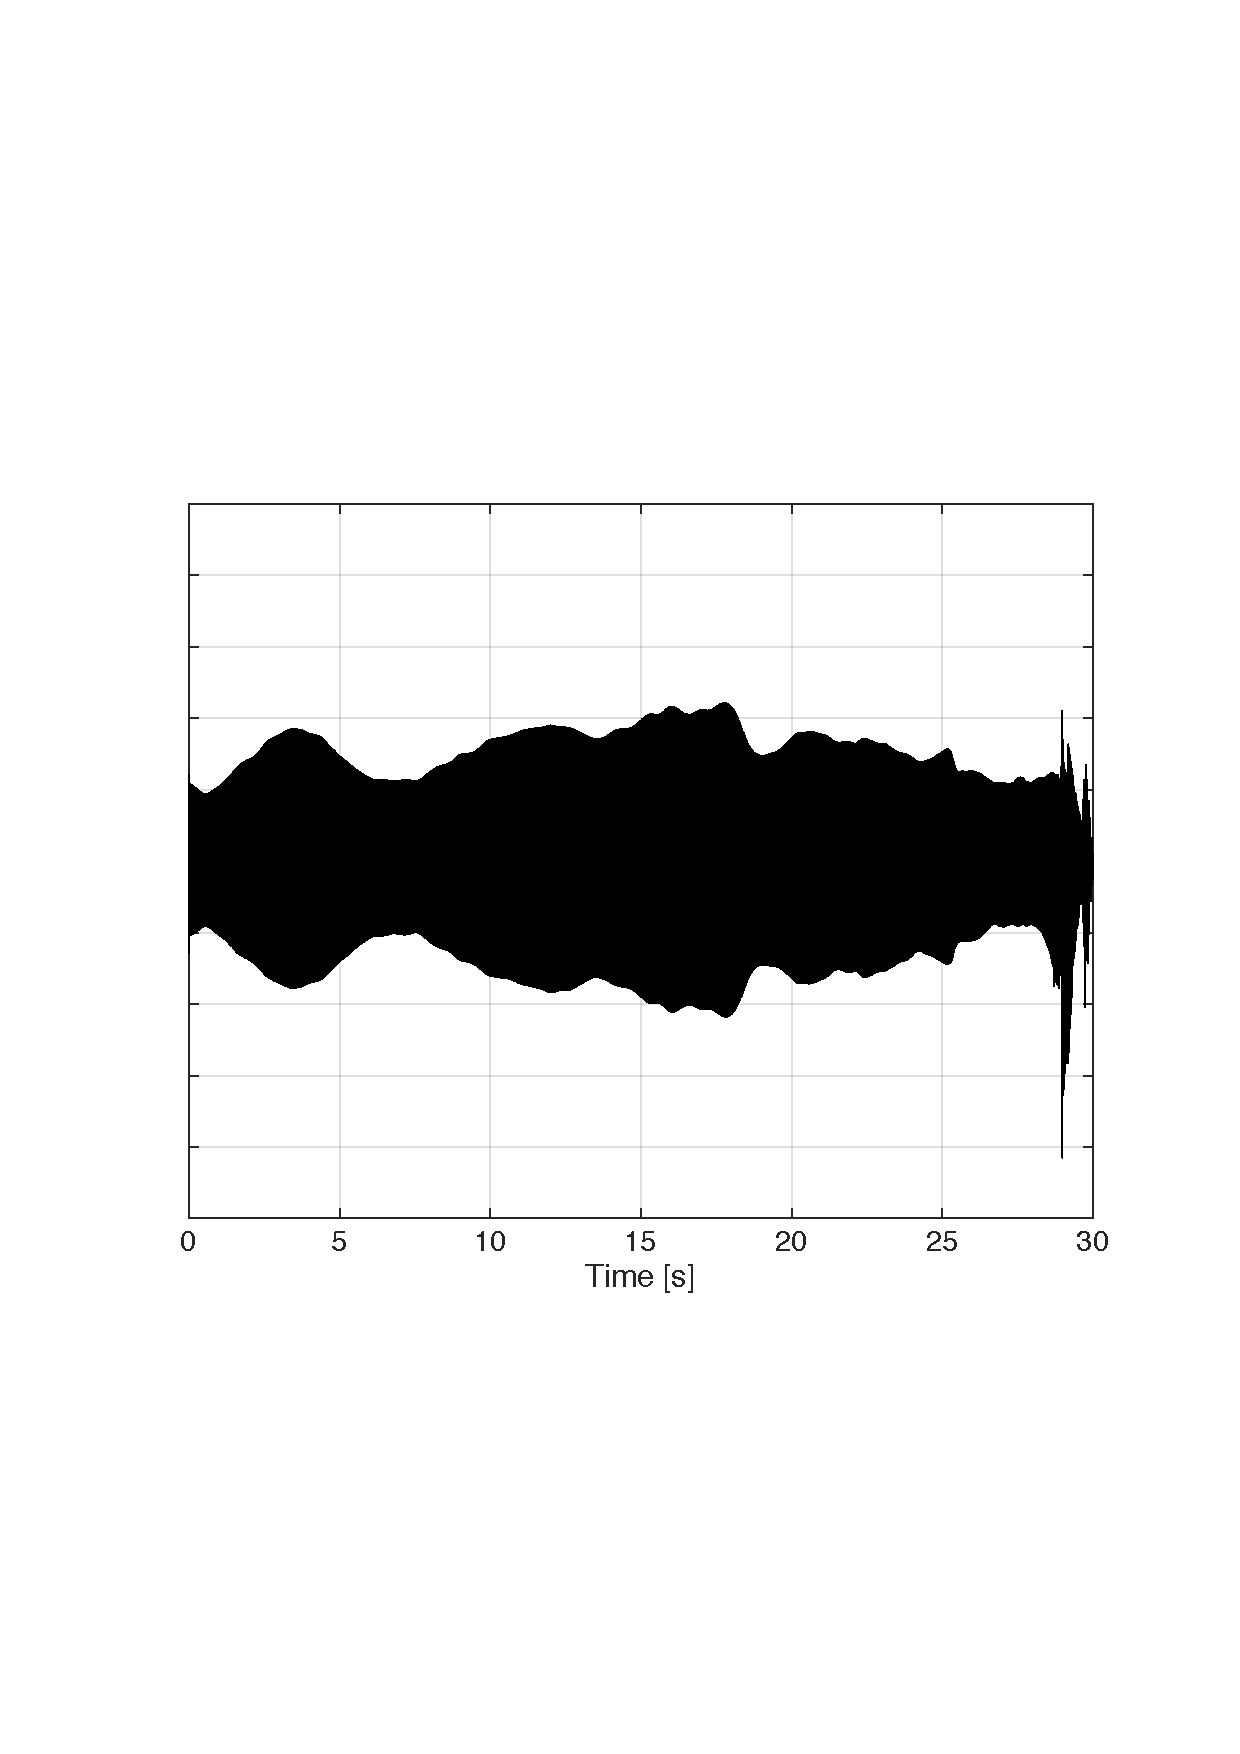
\includegraphics[width=1\textwidth]{figures/raw_microphone19.pdf}
	\caption{Sound pressure from microphone.}
	\label{fig:raw_microphone19}
\end{subfigure}
\caption{The measured data of (a) the vibration on the driver, (b) the vibration on the enclosure, and (c) the sound pressure from the microphone. Dataset 19.}
\label{fig:raw19}
\end{figure} 

Dataset 19 has the same characteristics as dataset 14, though with a more noticeable peak at 29 seconds for both the measurements from the driver and the microphone. In the last dataset shown in \autoref{fig:raw20}, the loudspeaker breaks down.


\begin{figure}[H]
\centering
\begin{subfigure}[t]{0.335\textwidth}
	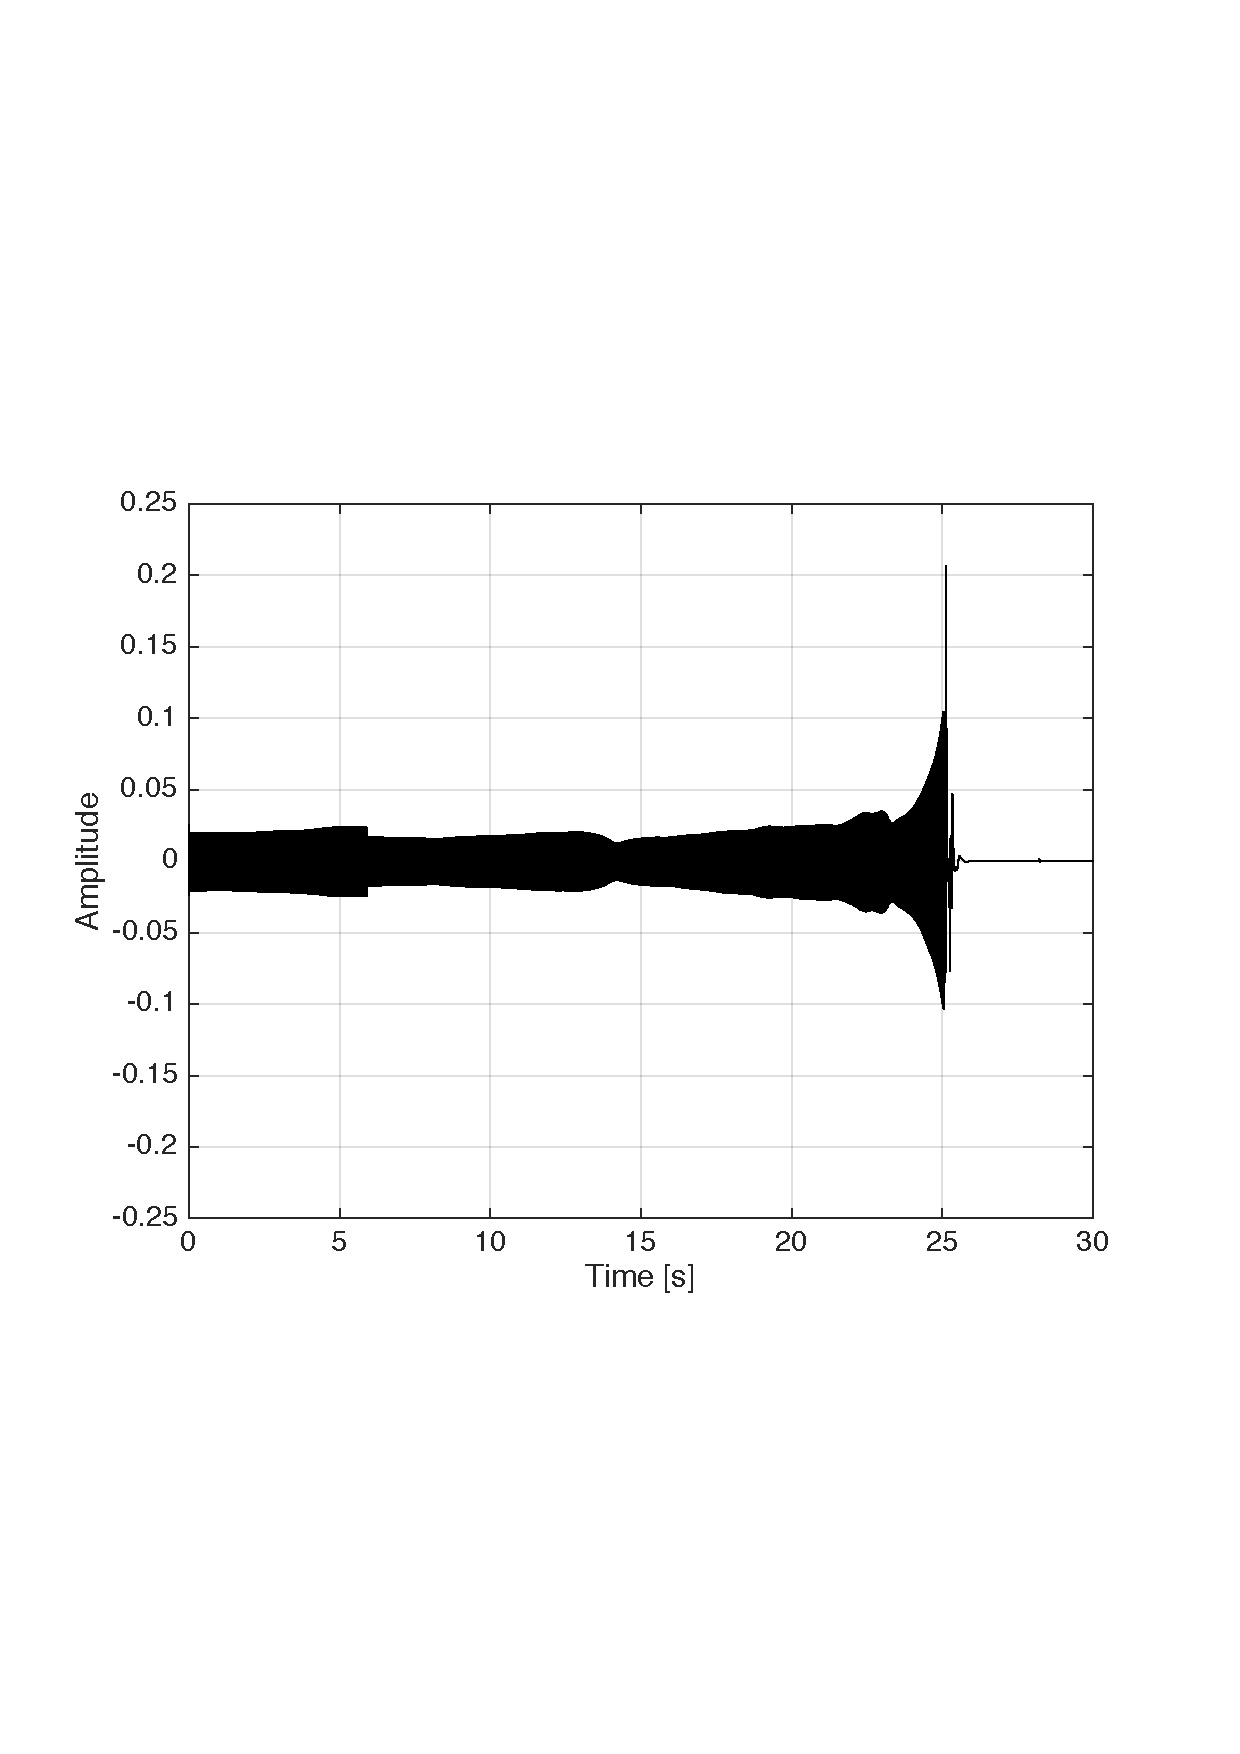
\includegraphics[width=1\textwidth]{figures/raw_driver20.pdf}
	\caption{Vibration from driver.}
	\label{fig:raw_driver20}
\end{subfigure}
\begin{subfigure}[t]{0.3\textwidth}
	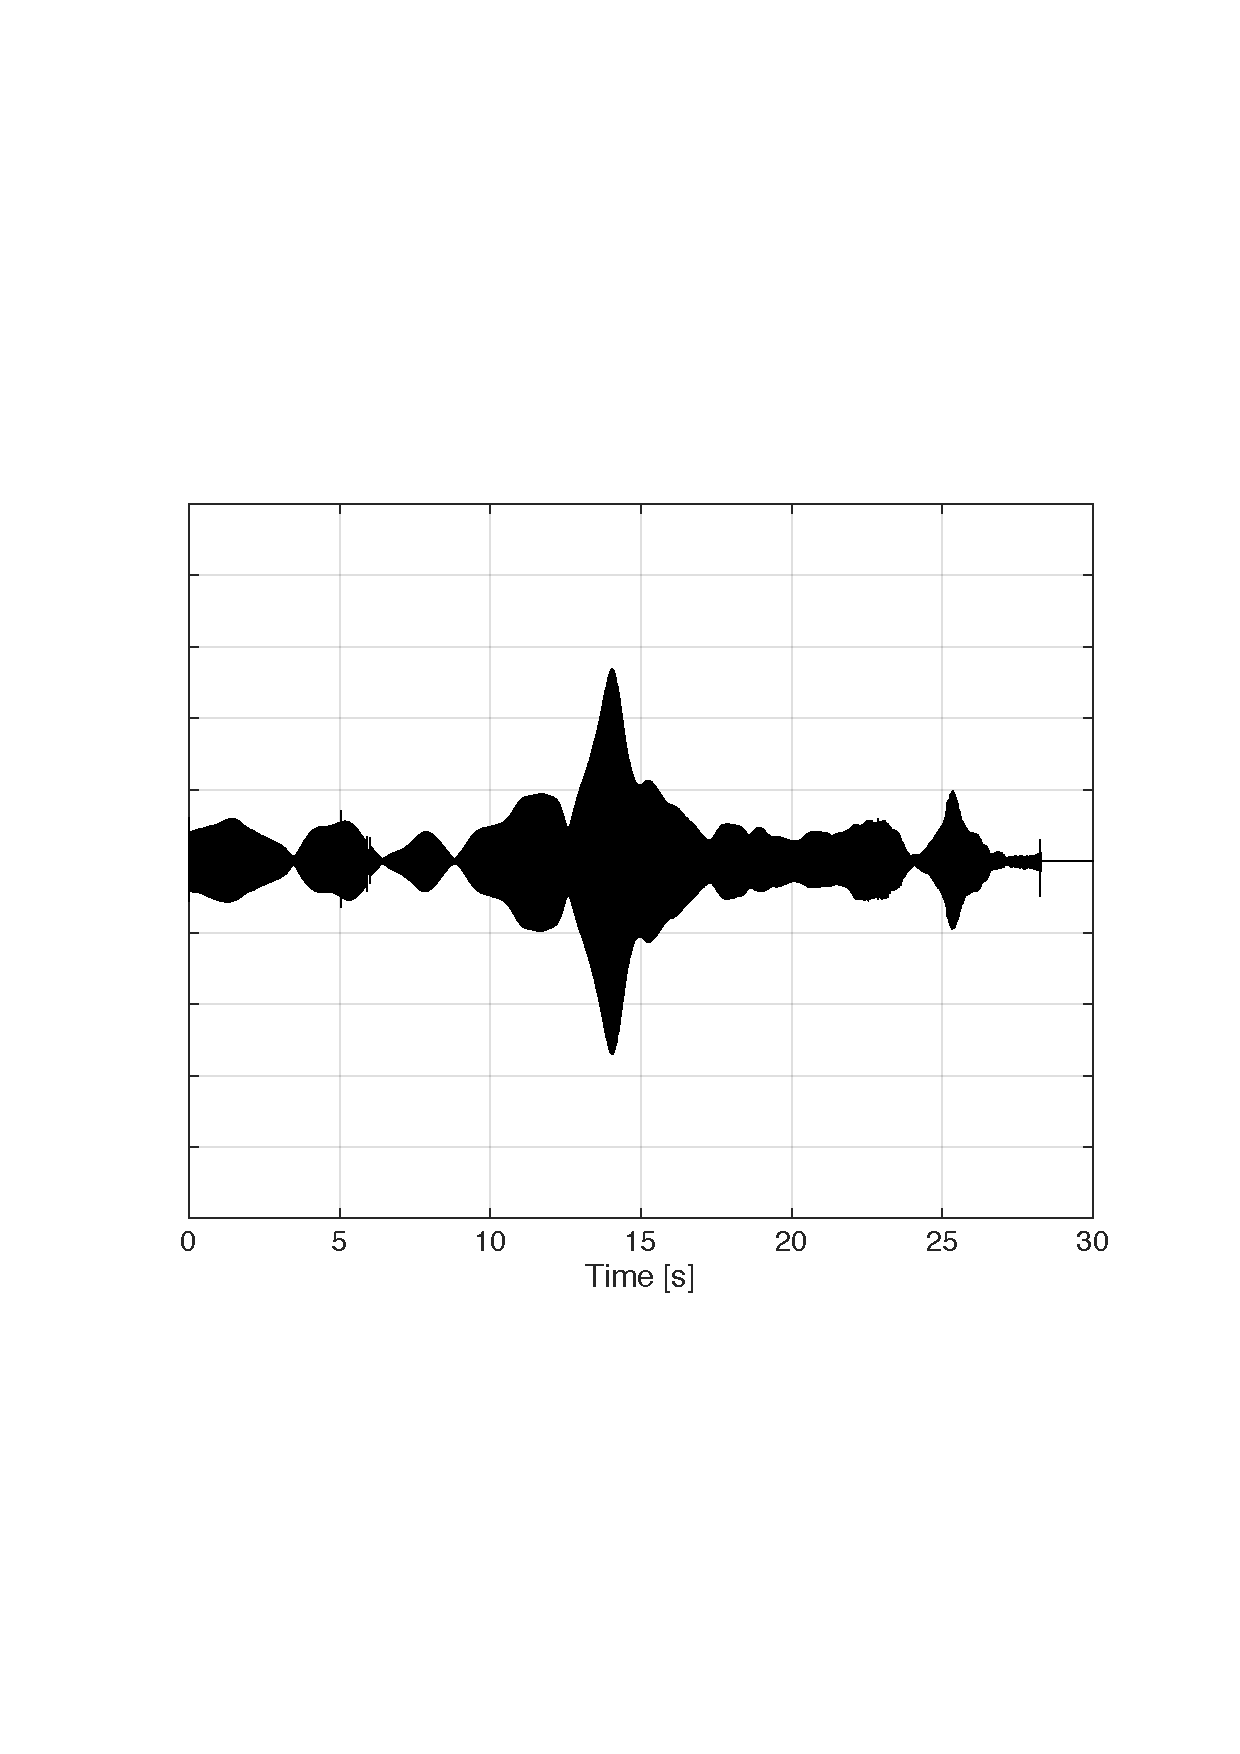
\includegraphics[width=1\textwidth]{figures/raw_enclosure20.pdf}
	\caption{Vibration from enclosure.}
	\label{fig:raw_enclosure20}
\end{subfigure}
\begin{subfigure}[t]{0.3\textwidth}
	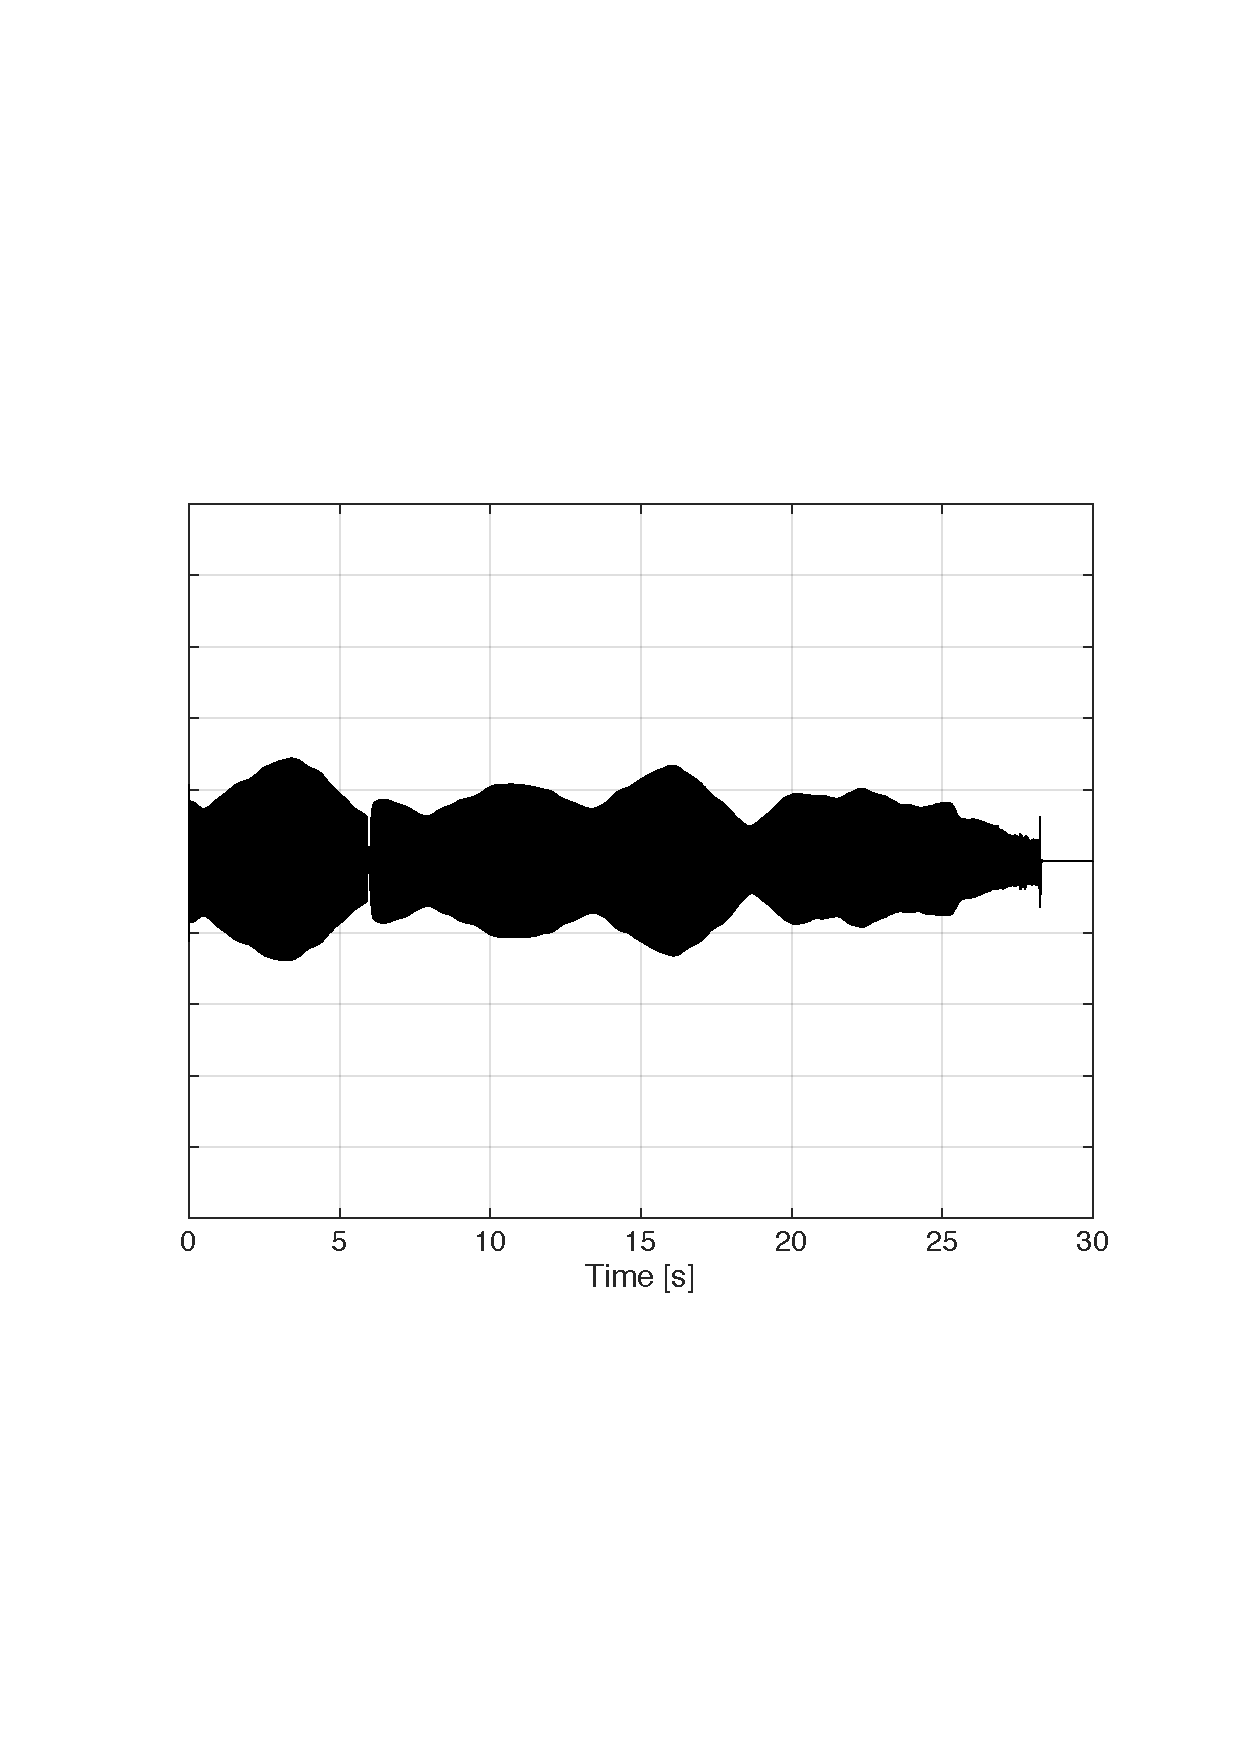
\includegraphics[width=1\textwidth]{figures/raw_microphone20.pdf}
	\caption{Sound pressure from microphone.}
	\label{fig:raw_microphone20}
\end{subfigure}
\caption{The measured data of (a) the vibration on the driver, (b) the vibration on the enclosure, and (c) the sound pressure from the microphone. Dataset 20.}
\label{fig:raw20}
\end{figure} 

As seen in \autoref{fig:raw_driver20} the loudspeaker unit breaks down at the mechanical resonance frequency for the driver. The reason to why vibrations on the enclosure and sound pressure are still presentthe  after 25 seconds is because the other loudspeaker unit did not entirely break down. Since the loudspeaker unit broke down at the mechanical driver resonance frequency, it would be relevant to examine if there is any correlation as such.




% Formål

% Råt Data

% Frekvensrespons
% - Konklusion: Ikke muligt at detektere tegn på at højtaleren har nået grænsen
% - Accelerometeret kan bruges til at estimere lydtrykket

% Harmonisk forvrængning
% - Der er tydelige tegn på øget harmonisk forvrængning, når lydstyrken øges.
% - Det er dog ikke muligt at måle harmonisk forvrængning, når der er tale om musik og derfor er det ikke muligt at udvinde information om harmonisk forvrængning

% Slag detektering
% - Undersøger et givet punkt i målingerne, der ligner slag mod driveren.
% - Spektralanalyser i området viser at der sker en betydelig energinieauet i lave frekvensen.
% - Da amplitude forøgelsen ikke er forbeholdt harmoniske frekvenser, må det antages at udslagene har er i impulser der 


% Conclusion: 
% - The vibration do not affect the distortion
% - The vibration can however be used as a tool to determine the sound pressure level since there is a strong correlation between the amount of vibration and sound pressure.
% - The analysis of the hits suggest that it is possible to detect these hits by measurering very low frequenct frequencies and determine the energy increase

% Further investigation
% - Investigate the impulse response of the loudspeaker
% - Investigate if there is a if the break of the loudspeaker unit was due to the amount of vibration at the resonance frequency.






